\documentclass[12pt, a4paper]{article}

% ── Geometry and spacing ──────────────────────────────────────────────────────
\usepackage[top=2.5cm, bottom=2.5cm, left=2.8cm, right=2.8cm]{geometry}
\usepackage{setspace}
\onehalfspacing

% ── Prevent automatic word hyphenation ───────────────────────────────────────
\hyphenpenalty=10000
\exhyphenpenalty=10000
\sloppy

% ── Core packages ─────────────────────────────────────────────────────────────
\usepackage{graphicx}
\usepackage{booktabs}
\usepackage{array}
\usepackage{tabularx}
\usepackage{multirow}
\usepackage{amsmath}
\usepackage{float}
\usepackage{caption}
\usepackage{subcaption}
\usepackage{parskip}
\usepackage{microtype}
\usepackage{natbib}
\usepackage[hidelinks]{hyperref}

% ── Caption formatting ────────────────────────────────────────────────────────
\captionsetup{font=small, labelfont=bf, skip=6pt}

% ── Section spacing ───────────────────────────────────────────────────────────
\usepackage{titlesec}
\titlespacing*{\section}{0pt}{14pt}{6pt}
\titlespacing*{\subsection}{0pt}{10pt}{4pt}

\begin{document}

% ── Title page ────────────────────────────────────────────────────────────────
\begin{titlepage}
\centering
\vspace*{2cm}
{\Large\bfseries Deep Learning for Prostate Histopathology\\[6pt]
Classification, Progression Modelling, and Structural Interpretation\\[6pt]
Across Multiple Imaging Domains\par}
\vspace{1.5cm}
{\large Rabin Bajagain\par}
\vspace{0.5cm}
{\normalsize Precision Oncology\\[3pt]
April 2026\par}
\vspace{3cm}
\begin{abstract}
\noindent
Gleason grading of prostate tissue is one of the most important steps in determining
how dangerous a cancer is. Pathologists assign grades by looking at tissue structure
under a microscope, but this process is slow and can vary between experts. In this
study, we trained a convolutional neural network to classify prostate tissue patches
into five categories and then used the internal representations learned by the network
to investigate how Gleason grades relate to each other. We found that the model reached
94.4 percent macro F1 on one imaging cohort and 95.4 percent on a second independent
cohort, compared to a majority-class baseline of 6.7 percent macro F1 on a balanced
five-class problem. Analysis of the network features showed that grades 3 through 5 form
a continuous and ordered structure in the learned feature space, with grade 4 acting as
a dispersed transition region. When we tested the models on unseen imaging cohorts,
performance dropped to around 40 to 56 percent, revealing that the models had partially
learned imaging artefacts rather than tissue biology. Stain normalisation did not
recover performance. We then extracted hand-crafted structural features from the raw
images and confirmed that lumen fraction, nuclear crowding, and tissue texture align
with the grade ordering, with 9 of 12 features showing statistically significant
Spearman correlations after Bonferroni correction. A new Structural Accessibility Index
captures how open or compact a tissue patch is, which has direct relevance to drug
delivery in tumours. These findings show that deep learning can build meaningful internal
models of prostate tissue biology, but that generalising across imaging sites remains
a critical unsolved challenge.
\end{abstract}
\end{titlepage}

\tableofcontents
\newpage

% ─────────────────────────────────────────────────────────────────────────────
\section{Introduction}
% ─────────────────────────────────────────────────────────────────────────────

Prostate cancer is the second most common cancer diagnosed in men globally, with
around 1.4 million new cases each year \citep{campanella2019}. One of the most
important tools doctors use to predict how a prostate cancer will behave is the
Gleason grading system. A pathologist examines a biopsy sample and assigns a grade
based on how the glandular structures in the tissue look. Grade 3 tumours have
recognisable glands, grade 4 glands begin to fuse or lose their shape, and grade
5 tumours have lost all glandular architecture and form solid sheets of cells. The
higher the grade, the more aggressive the cancer tends to be \citep{epstein2016}.

Manual grading is labour intensive. A pathologist must examine hundreds of tissue
patches from a single biopsy slide. The interpretation can also differ between
pathologists, particularly for grade 4 tumours where the boundaries are less
clearly defined. These limitations have motivated researchers to explore whether
computers can help by automating some or all of the grading process \citep{litjens2017}.

Deep learning, and convolutional neural networks in particular, have transformed
the field of computational pathology in recent years \citep{kather2020}. Networks
trained on large image datasets can learn to recognise the visual patterns that
define different tissue categories without being explicitly told which visual
features to look for. Once trained, such a network can process thousands of patches
in seconds.

Most published studies report strong performance when a model is tested on images
from the same scanner or institution where it was trained. The more challenging
and clinically relevant question is whether a model trained in one hospital can be
used reliably in a different one, where the staining protocol and imaging equipment
may differ. This cross-site or cross-domain problem is one of the central challenges
in making digital pathology tools usable in practice.

This study investigates prostate tissue classification across three independent
imaging cohorts. We train a classifier, examine the internal feature representations
it learns, test it on unseen imaging domains, and then attempt to explain the learned
representations in terms of measurable tissue structure. The goal is to understand
both what the model learns and where it fails.

% ─────────────────────────────────────────────────────────────────────────────
\section{Dataset and Data Preparation}
% ─────────────────────────────────────────────────────────────────────────────

\subsection{Imaging Cohorts}

Three imaging cohorts were used in this study. The first two, referred to here as
Cohort A and Cohort B, served as the primary training and evaluation datasets. The
third, referred to as the NTU cohort, was used exclusively as an external test set
and was never seen during training. All images are square patches of 251 by 251
pixels in the Tagged Image File Format, derived from whole-slide prostate biopsies
stained with haematoxylin and eosin.

Each patch belongs to one of five tissue categories. Stroma is fibromuscular tissue
without glandular structures. Normal refers to benign prostate glands. Grades 3,
4, and 5 correspond to the three clinically significant Gleason grades. A summary
of the dataset distribution is given in Table~\ref{tab:dataset}.

\begin{table}[H]
\centering
\caption{Patch counts per tissue class and data split for each cohort. Cohort A
and Cohort B have identical distributions. The NTU cohort was used only for
external testing.}
\label{tab:dataset}
\begin{tabular}{lrrrrr}
\toprule
\textbf{Class} & \textbf{Train} & \textbf{Validation} & \textbf{Test (A/B)} & \textbf{Test (NTU)} \\
\midrule
Stroma & 680 & 120 & 200 & 200 \\
Normal & 680 & 120 & 200 & 200 \\
Grade 3 & 680 & 120 & 200 & 200 \\
Grade 4 & 680 & 120 & 200 & 200 \\
Grade 5 & 425 &  75 & 200 & 200 \\
\midrule
\textbf{Total} & \textbf{3145} & \textbf{555} & \textbf{1000} & \textbf{1000} \\
\bottomrule
\end{tabular}
\end{table}

\subsection{Data Splitting}

The validation set was created by randomly sampling 15 percent of the training pool
for each class separately, ensuring proportional class representation. This was done
using a stratified random split with a fixed random seed to allow reproducibility.
The test set was kept entirely separate and was not used during training or for any
model selection decision. We verified that no image path appears in both the training
and test sets.

\subsection{Class Imbalance}

Grade 5 patches are less common in the dataset, with 500 training patches compared
to 800 for other classes. To avoid the model ignoring this class, we applied
inverse-frequency class weights during training. The weight assigned to grade 5
was approximately 1.48 times larger than the weight for other classes.

\subsection{Image Preprocessing and Augmentation}

All patches were resized from 251 to 224 pixels to match the input requirements of
the network. Pixel values were normalised using the mean and standard deviation of
the ImageNet dataset, which is standard practice when using a network that was
initially trained on natural images. During training, each patch was randomly
flipped horizontally or vertically, rotated by 90 degrees, and subjected to small
random changes in brightness and contrast. These augmentations were applied to
expose the model to the natural variability in how tissue can be oriented and how
staining intensity can vary between slides.

% ─────────────────────────────────────────────────────────────────────────────
\section{Model Architecture and Training}
% ─────────────────────────────────────────────────────────────────────────────

\subsection{Network Architecture}

We used EfficientNet-B2 \citep{efficientnet} as the backbone for classification.
This network was chosen because its native input size of 260 pixels is very close
to the 251-pixel patch size in this dataset, meaning the patches require almost no
rescaling. EfficientNet-B2 has approximately 9 million parameters, which is large
enough to capture the morphological detail needed to distinguish Gleason grades
but small enough to train in a reasonable time. All layers of the network were
unfrozen from the first training epoch, allowing the entire network to adapt to
histology images.

The final classification layer was replaced with a linear layer mapping the
1408-dimensional feature vector to five output classes. The 1408-dimensional
representation produced just before this layer was retained for all downstream
analysis of the learned feature space.

\subsection{Training Configuration}

The network was trained using the AdamW optimiser with a learning rate of
$3\times10^{-4}$ and weight decay of $10^{-4}$. The learning rate schedule
consisted of a linear warmup over the first five epochs followed by cosine
decay. Training was stopped early if the macro F1 score on the validation set
did not improve for twelve consecutive epochs. The primary evaluation metric
was macro F1, which gives equal weight to all five classes regardless of their
sample count.

% ─────────────────────────────────────────────────────────────────────────────
\section{Classification Performance}
% ─────────────────────────────────────────────────────────────────────────────

\subsection{Baseline Context}

Before examining model performance, it is important to establish a lower bound.
A majority-class baseline that always predicts the most frequent class achieves
20 percent accuracy on a balanced five-class problem and a macro F1 of approximately
6.7 percent, because it scores zero on the four classes it never predicts. All
reported performance figures should be interpreted relative to this lower bound.

\subsection{Overall Results}

The classifier reached a macro F1 score of 94.4 percent on the Cohort A test set
and 95.4 percent on the Cohort B test set. Both scores were achieved without any
hyperparameter tuning between cohorts. The same configuration was used for both.
Per-class results are shown in Table~\ref{tab:classification}.

\begin{table}[H]
\centering
\caption{Per-class precision, recall, and F1 on the test sets of Cohort A and
Cohort B. Macro F1 treats all five classes equally.}
\label{tab:classification}
\begin{tabular}{lcccccc}
\toprule
 & \multicolumn{3}{c}{\textbf{Cohort A}} & \multicolumn{3}{c}{\textbf{Cohort B}} \\
\cmidrule(lr){2-4} \cmidrule(lr){5-7}
\textbf{Class} & \textbf{Prec.} & \textbf{Recall} & \textbf{F1} & \textbf{Prec.} & \textbf{Recall} & \textbf{F1} \\
\midrule
Stroma  & 0.976 & 1.000 & 0.988 & 0.961 & 0.980 & 0.970 \\
Normal  & 0.980 & 1.000 & 0.990 & 0.985 & 0.995 & 0.990 \\
Grade 3 & 0.956 & 0.980 & 0.968 & 0.979 & 0.945 & 0.962 \\
Grade 4 & 0.915 & 0.810 & 0.859 & 0.900 & 0.945 & 0.922 \\
Grade 5 & 0.895 & 0.935 & 0.914 & 0.948 & 0.905 & 0.926 \\
\midrule
\textbf{Macro F1} & & & \textbf{0.944} & & & \textbf{0.954} \\
\bottomrule
\end{tabular}
\end{table}

Training curves for both cohorts are shown in Figure~\ref{fig:training}. Both
models converge cleanly. The Cohort A model was stopped at epoch 11 and the
Cohort B model at epoch 21. In both cases, the training loss continued to fall
after the selected checkpoint. This is expected behaviour and the early stopping
criterion correctly identified the point at which validation performance stopped
improving.

\begin{figure}[H]
\centering
\begin{subfigure}[b]{0.48\textwidth}
  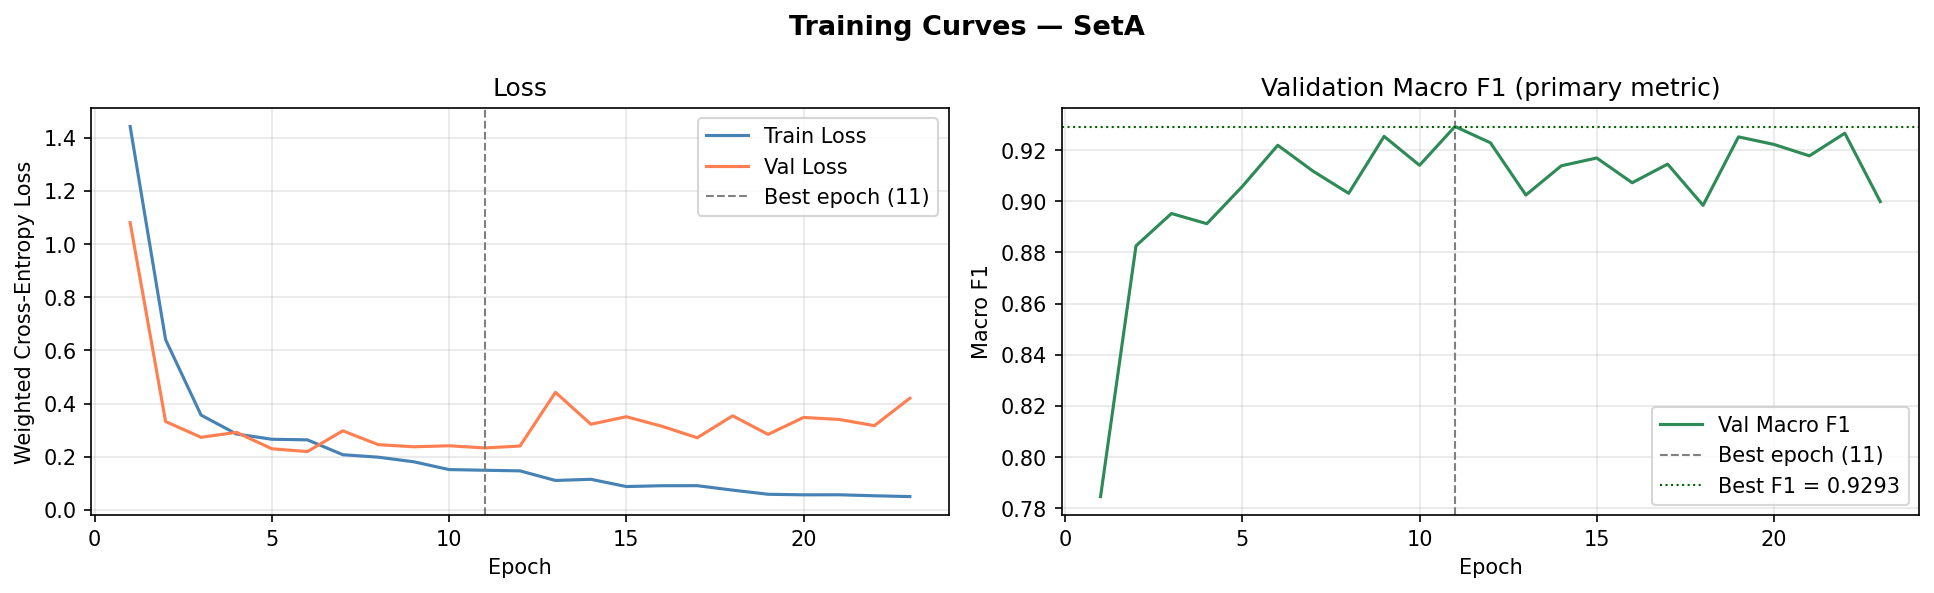
\includegraphics[width=\textwidth]{figures/training_curves_seta.png}
  \caption{Cohort A training curves}
\end{subfigure}
\hfill
\begin{subfigure}[b]{0.48\textwidth}
  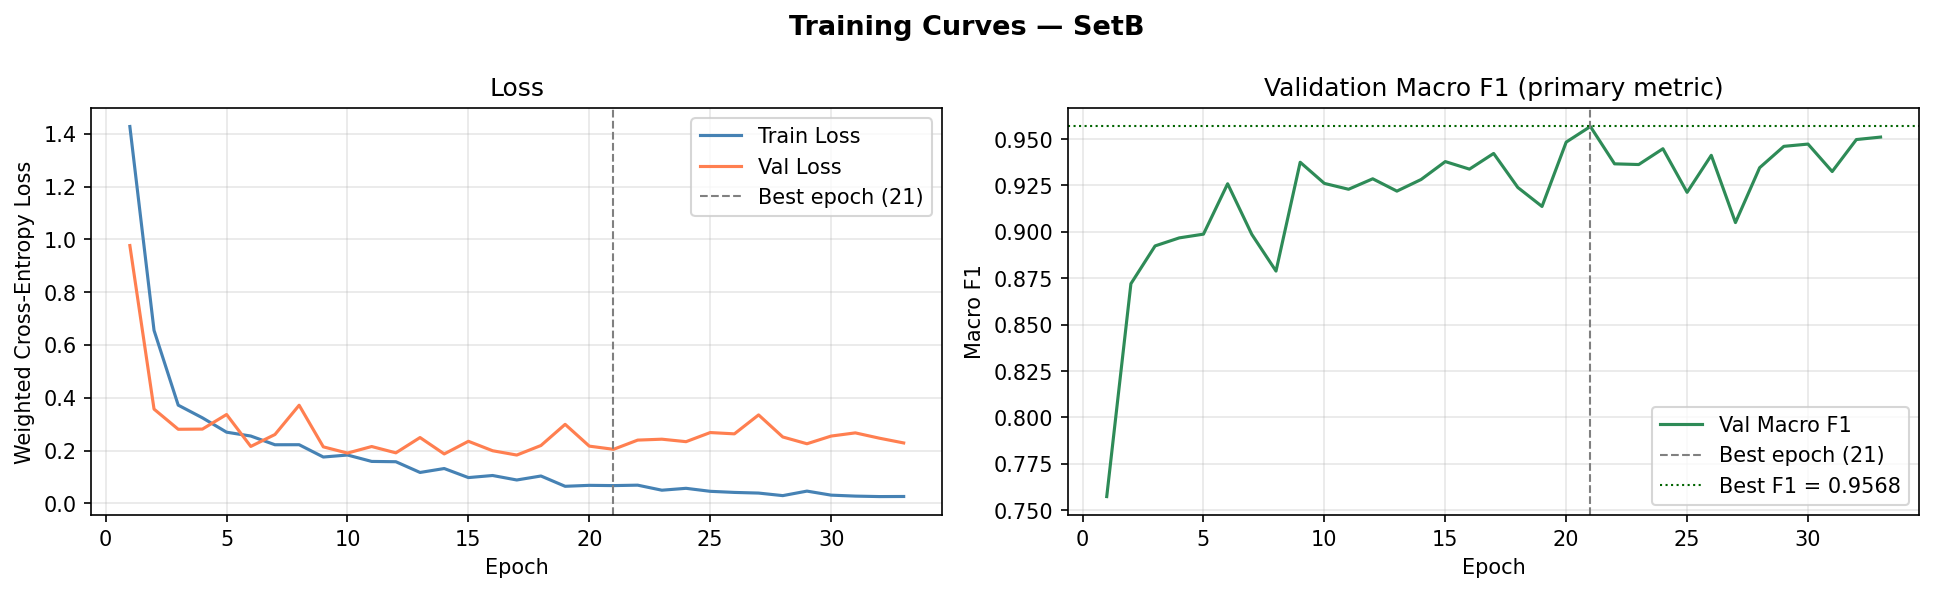
\includegraphics[width=\textwidth]{figures/training_curves_setb.png}
  \caption{Cohort B training curves}
\end{subfigure}
\caption{Training and validation loss and macro F1 across epochs for both
cohorts. The vertical dashed line marks the epoch selected by early stopping.
The widening gap between training and validation loss in Cohort A after epoch
11 indicates that the model would have overfit had training continued.}
\label{fig:training}
\end{figure}

\subsection{Confusion Patterns}

Confusion matrices for both cohorts are shown in Figure~\ref{fig:confusion}.
The most common error in both cohorts involves grades 4 and 5. In Cohort A,
22 out of 200 grade 4 patches were predicted as grade 5, accounting for 11 percent
of grade 4 patches. In Cohort B, 19 out of 200 grade 5 patches were predicted
as grade 4. This pattern is biologically expected. Grade 4 and grade 5 tissue
can look very similar because both involve significant loss of glandular
architecture. Benign classes, Stroma and Normal, are classified with very high
accuracy in both cohorts.

The grade 4 class had the lowest recall in Cohort A (81 percent) but the second
highest recall in Cohort B (94.5 percent). This 13-percentage-point difference
between cohorts suggests that the visual characteristics of grade 4 tissue vary
between the two imaging sites, which foreshadows the domain shift findings
discussed later.

\begin{figure}[H]
\centering
\begin{subfigure}[b]{0.48\textwidth}
  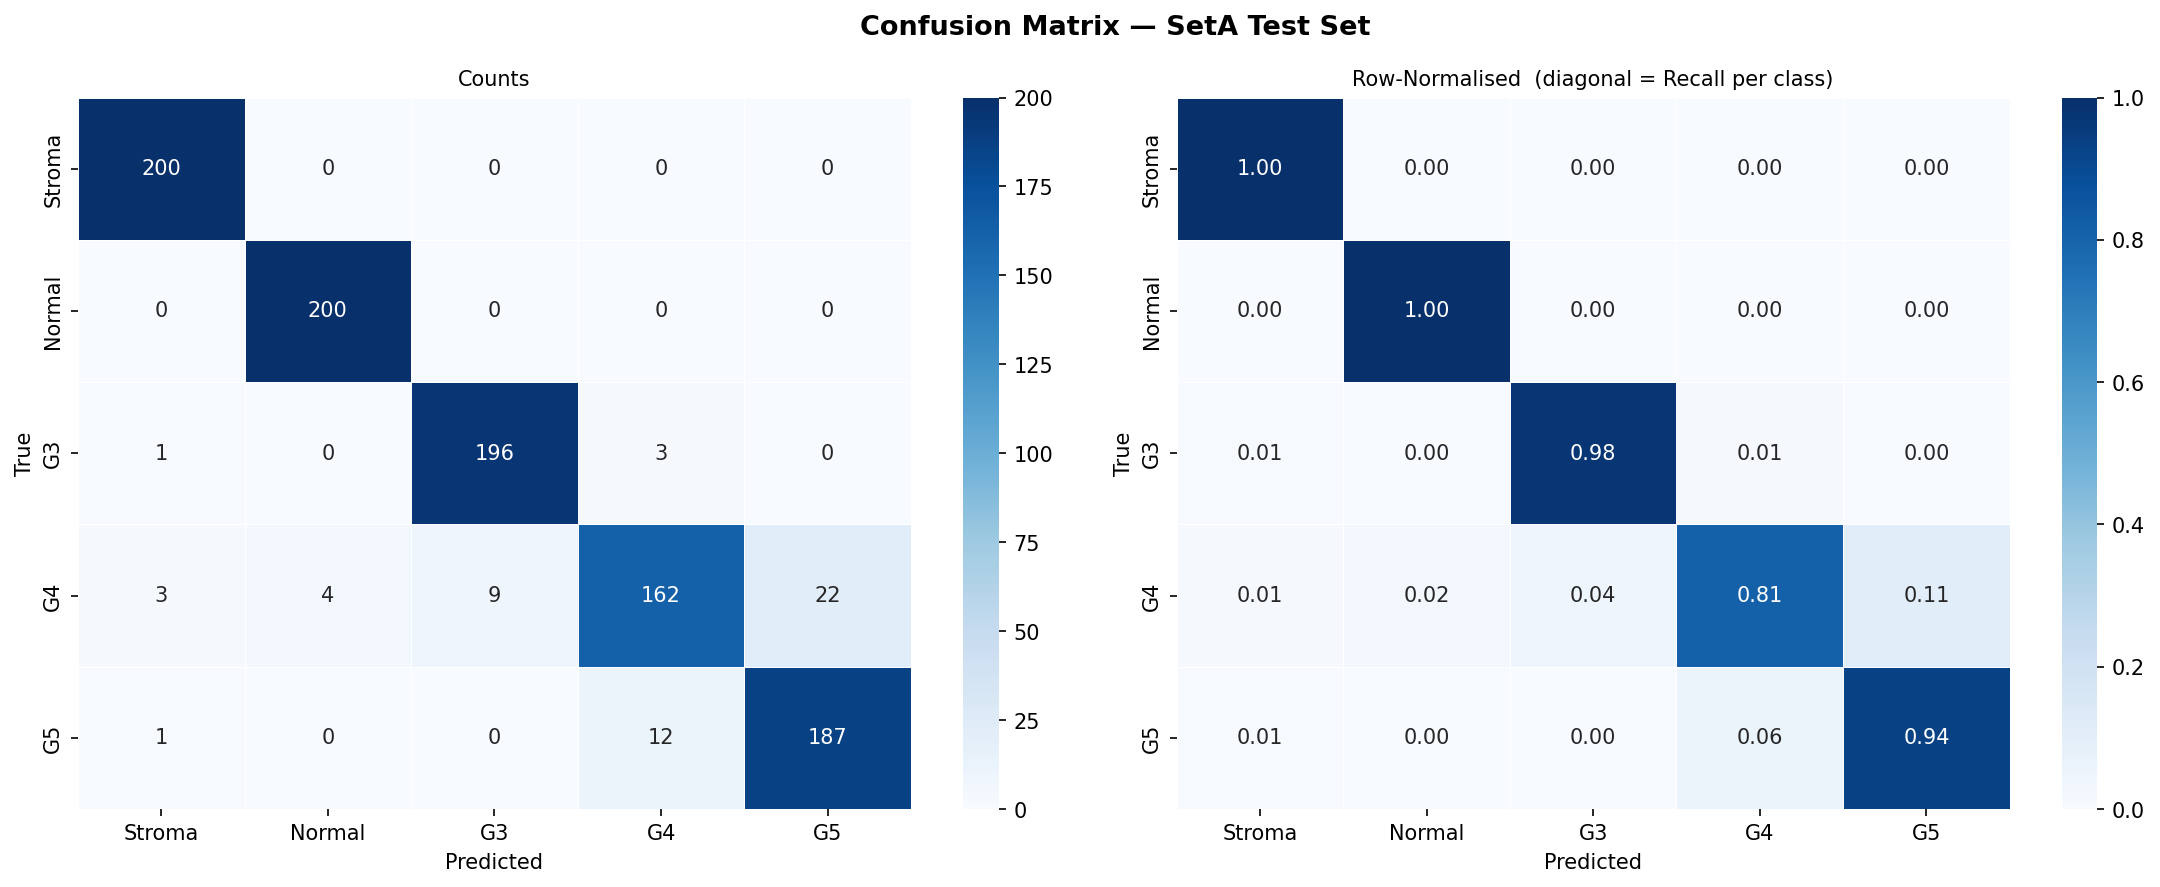
\includegraphics[width=\textwidth]{figures/confusion_seta.png}
  \caption{Cohort A}
\end{subfigure}
\hfill
\begin{subfigure}[b]{0.48\textwidth}
  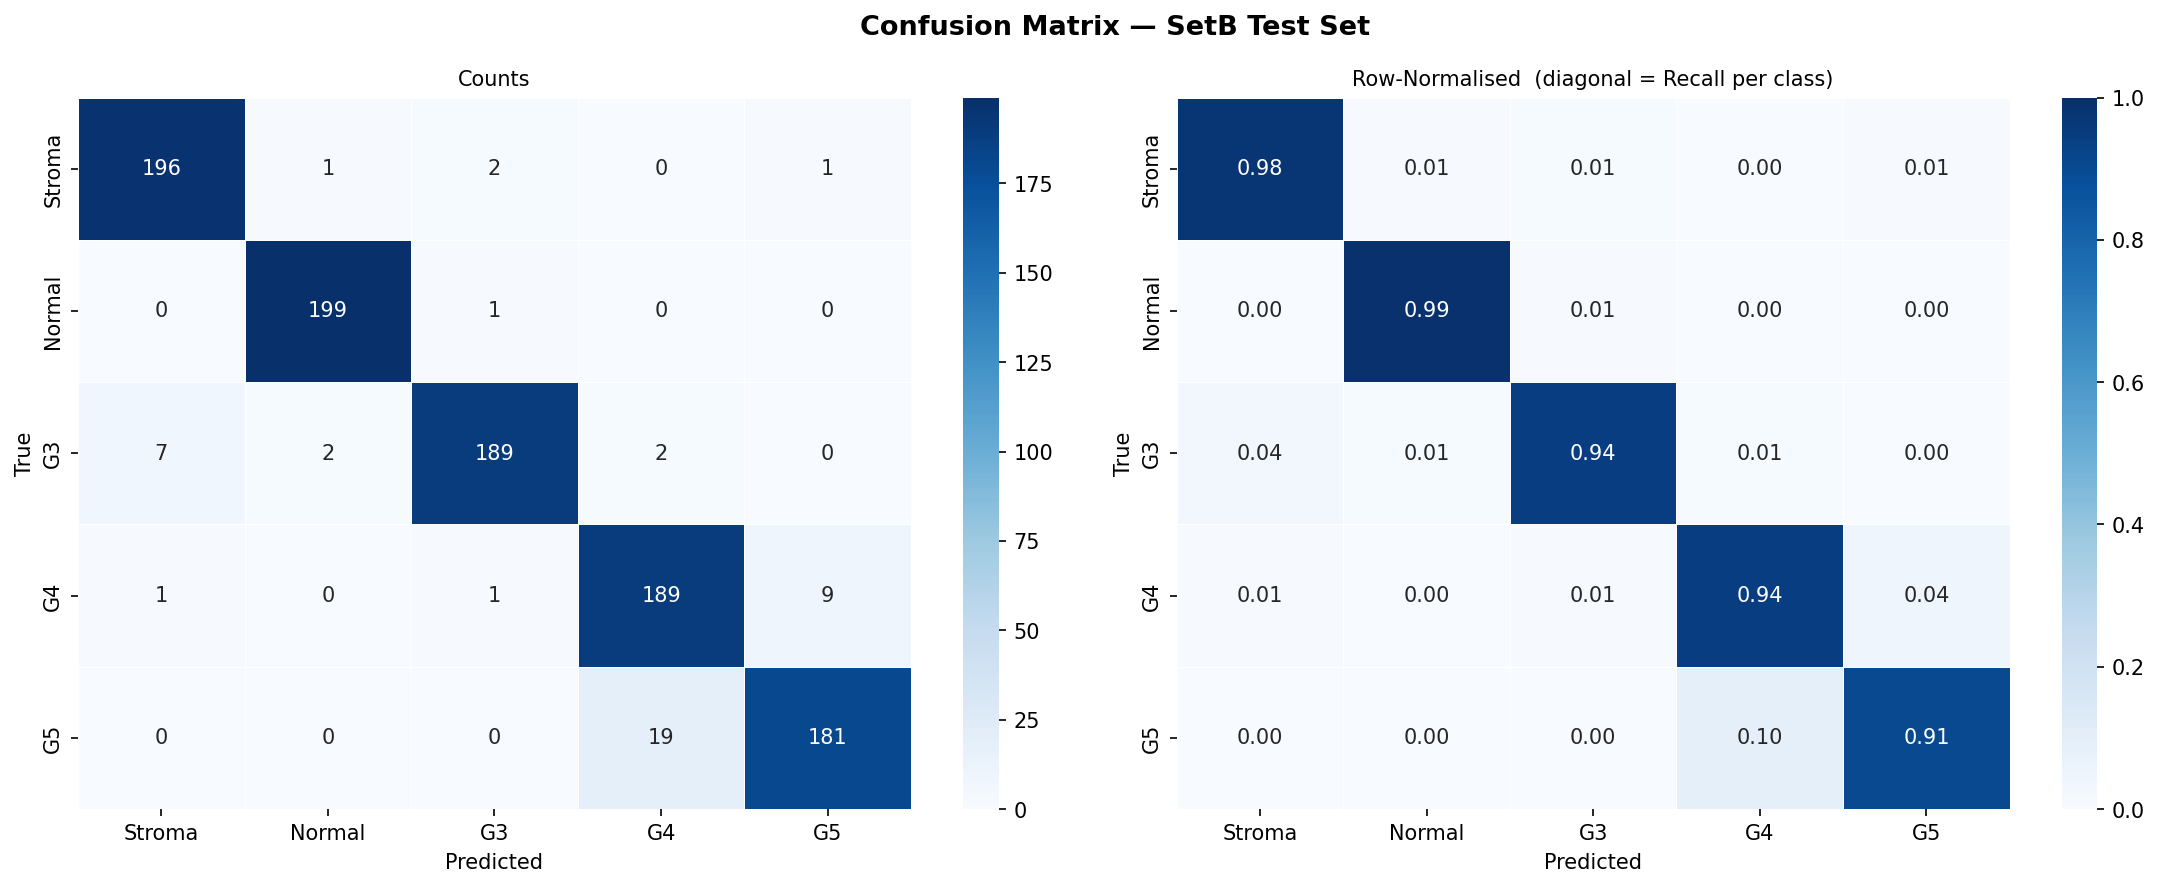
\includegraphics[width=\textwidth]{figures/confusion_setb.png}
  \caption{Cohort B}
\end{subfigure}
\caption{Normalised confusion matrices on the test sets. Each row represents the
true class and each column the predicted class. The diagonal shows recall per
class. The main off-diagonal errors concentrate at the grade 4 and grade 5
boundary.}
\label{fig:confusion}
\end{figure}

% ─────────────────────────────────────────────────────────────────────────────
\section{Feature Space and Disease Progression}
% ─────────────────────────────────────────────────────────────────────────────

\subsection{Embedding Extraction and Visualisation}

After training, we extracted the 1408-dimensional feature vector from each
test patch in all three cohorts, giving a total of 3000 vectors. These high-dimensional
representations were reduced to two dimensions using UMAP \citep{umap2018} for
visualisation. Before applying UMAP, the representations were compressed to
50 dimensions with PCA, which removes noise while preserving the main structure.

The resulting map is shown in Figure~\ref{fig:umap}. The tissue classes form
clearly separated clusters. Stroma and Normal occupy distinct regions away from
the cancer grades. Grades 3, 4, and 5 are arranged in a visually ordered sequence,
with grade 3 and grade 5 at opposite ends and grade 4 in between. The grade 4
cluster is notably more spread out than the grade 3 or grade 5 clusters, which
are relatively compact.

\begin{figure}[H]
\centering
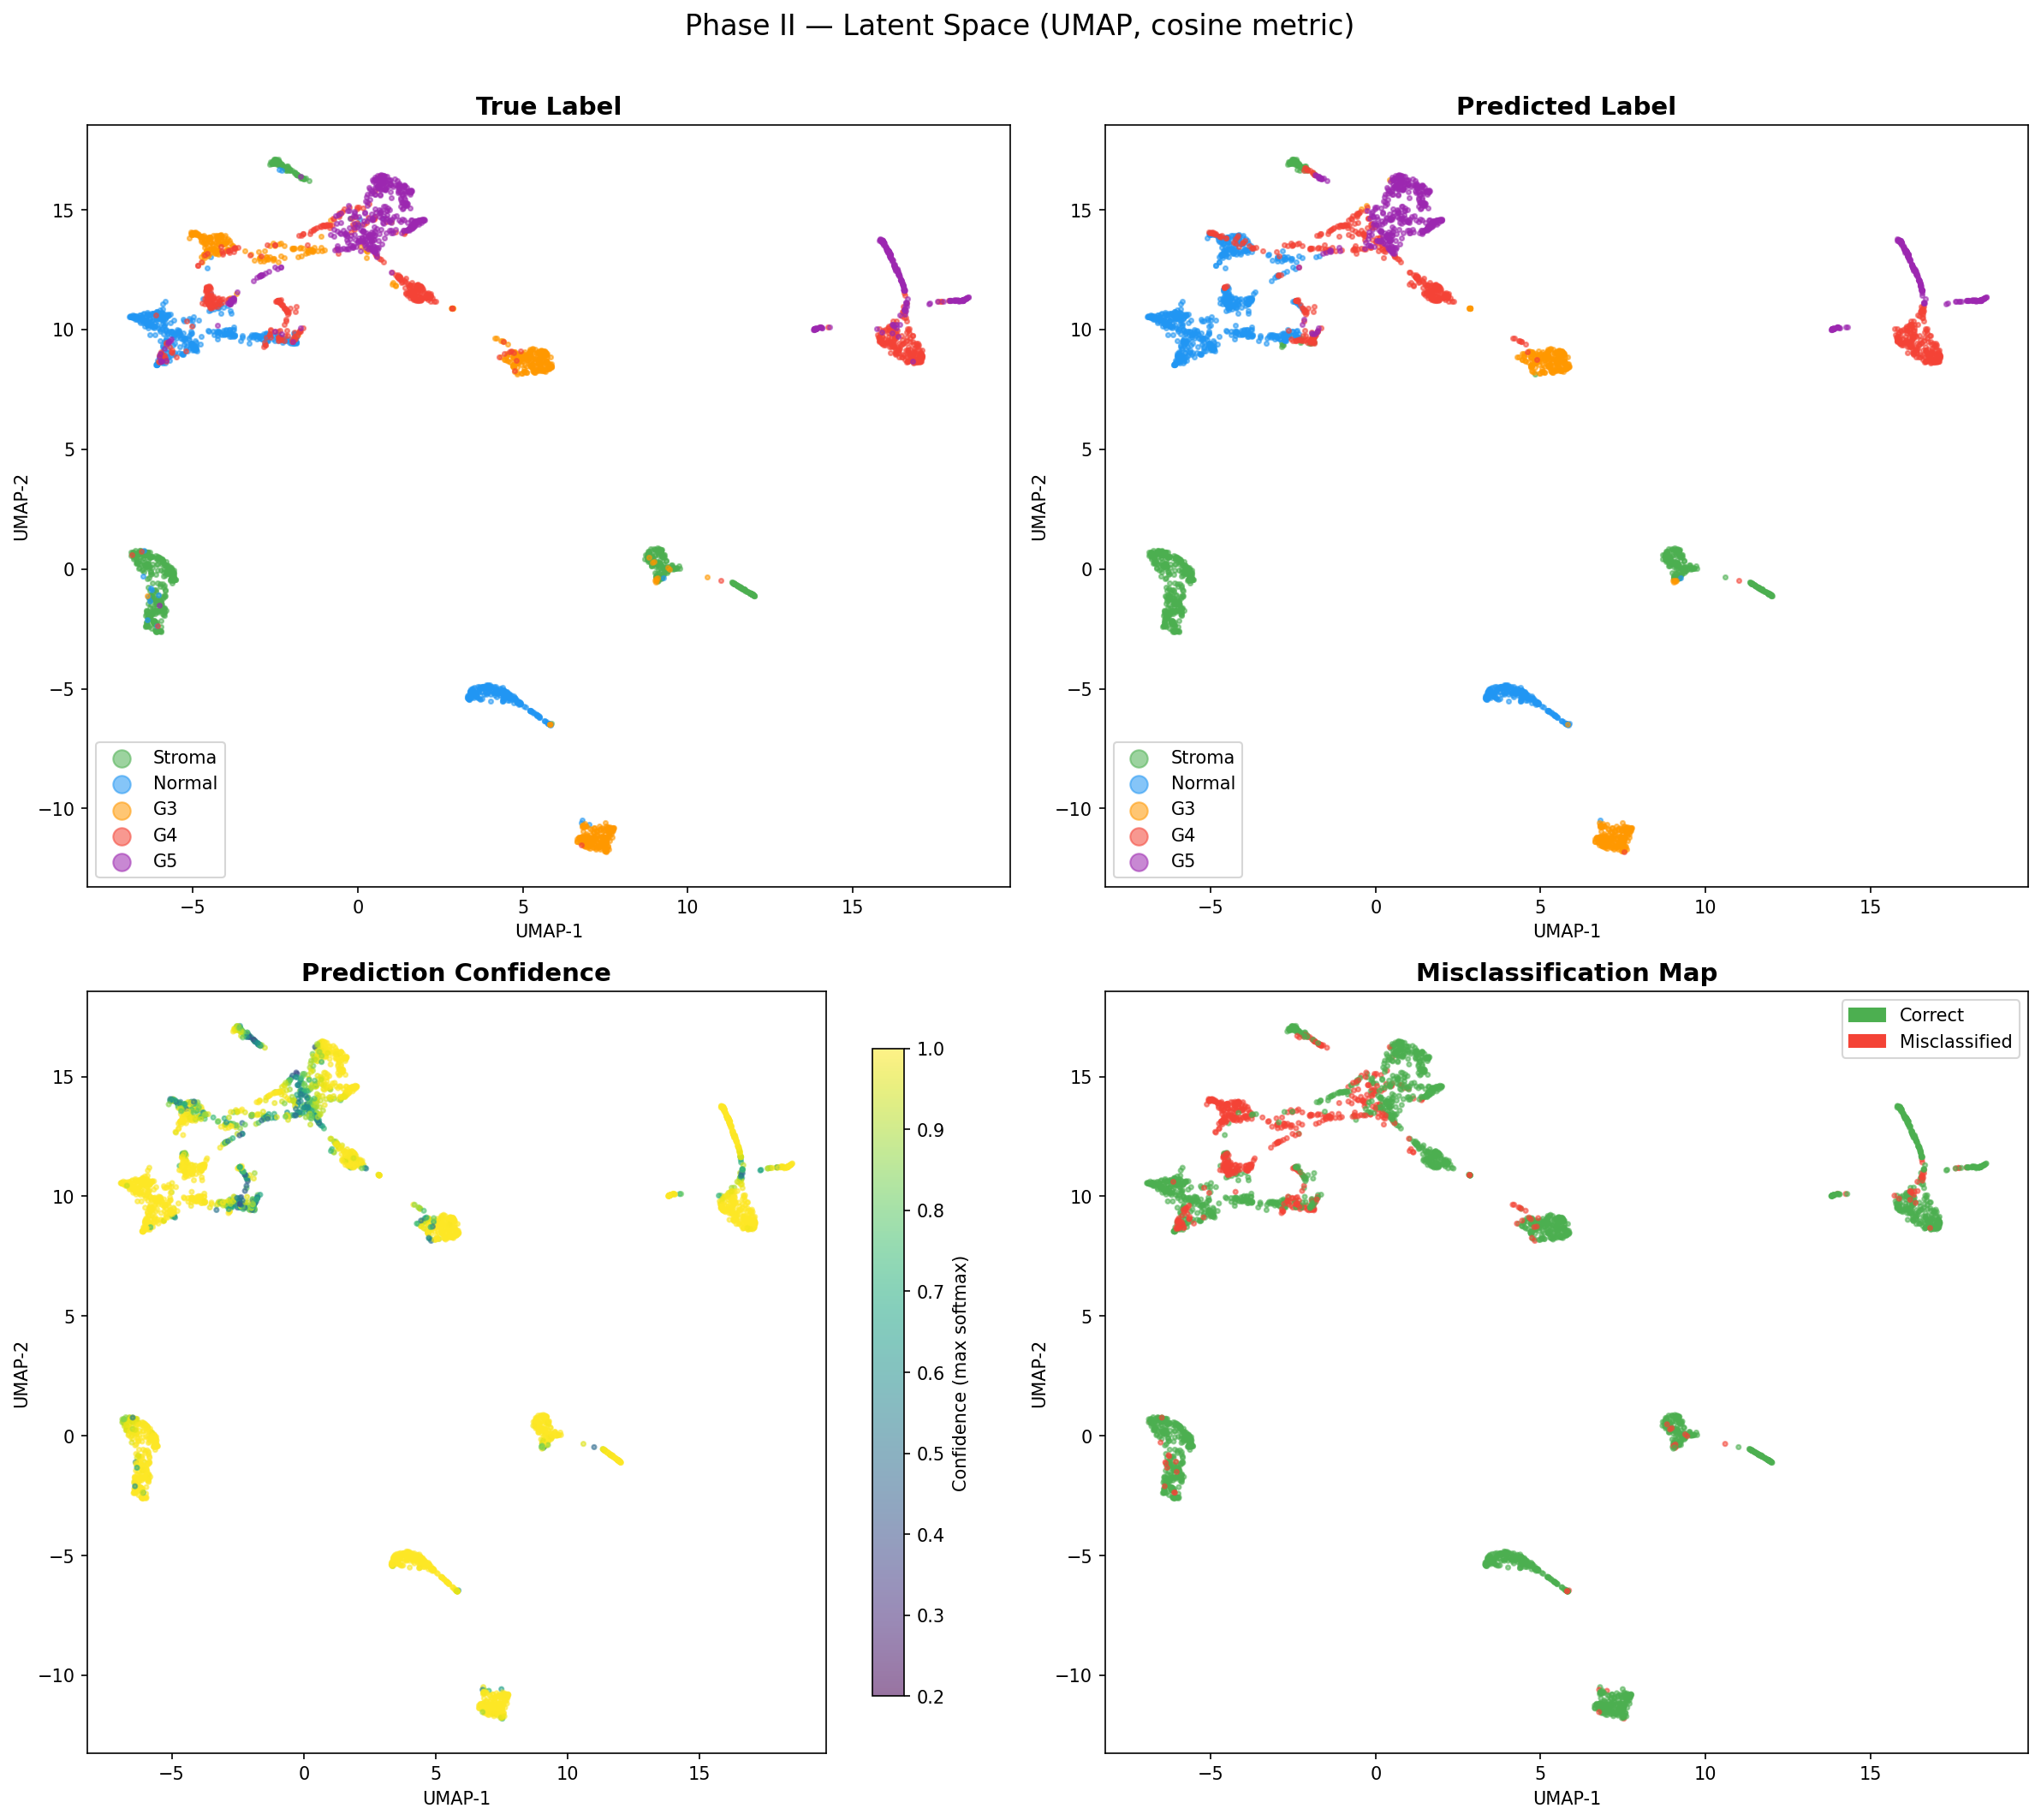
\includegraphics[width=0.92\textwidth]{figures/umap_4panel.png}
\caption{UMAP projection of the 1408-dimensional feature vectors from all 3000
test patches. Each panel shows the same map coloured by a different property.
Top left shows tissue class. Top right shows the source cohort. Bottom left
shows model confidence. Bottom right shows patches flagged as transition cases
near the grade boundaries.}
\label{fig:umap}
\end{figure}

\subsection{The Progression Axis}

To quantify the ordering observed in the UMAP map, we defined a progression axis
in the full 1408-dimensional feature space. This axis runs from the average feature
vector of grade 3 patches to the average feature vector of grade 5 patches. Each
patch is then assigned a progression score by projecting its feature vector onto
this axis.

Figure~\ref{fig:progression} shows the progression scores for all five tissue
classes. The three cancer grades are ordered correctly along the axis in all three
cohorts, with grade 3 having the lowest scores, grade 5 the highest, and grade 4
in between. The score distributions for grade 3 and grade 5 are relatively tight,
while the distribution for grade 4 is considerably wider, confirming that grade 4
occupies a transitional region in the feature space.

It is important to note a structural limitation of this construction. The axis is
defined by the grade 3 and grade 5 centroids, so the ordering of these two classes
at the respective ends of the axis is guaranteed by construction rather than
discovered independently. The meaningful empirical finding is that grade 4 projects
to an intermediate position between these fixed endpoints, and that its distribution
is substantially wider than either endpoint grade. This width reflects the known
architectural heterogeneity of grade 4 tissue.

One further observation is that Stroma and Normal tissue also project onto this axis
at intermediate positions rather than outside it. Stroma has a mean progression score
of about 10.6, which places it between grades 3 and 4. This is an artefact of the
axis construction. Because the axis is defined only by the endpoints (grade 3 and
grade 5), benign tissue that happens to share some feature dimensions with cancer
tissue will project to intermediate positions. The progression score should therefore
be interpreted only for cancer-grade patches.

\begin{figure}[H]
\centering
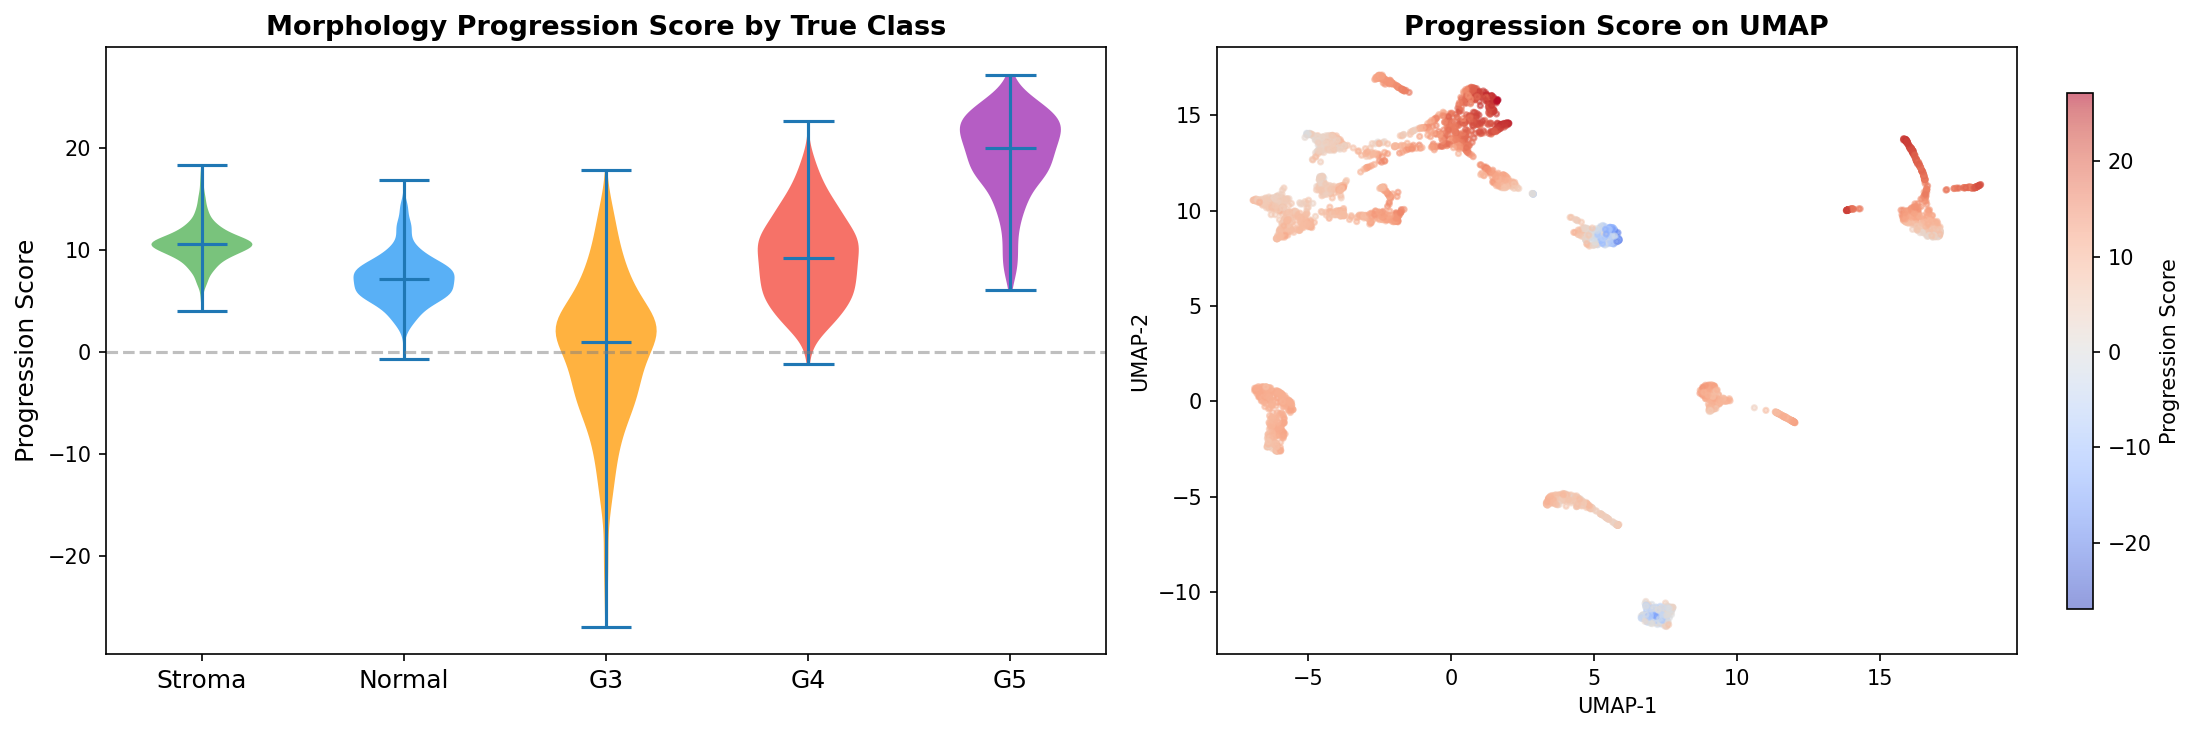
\includegraphics[width=0.85\textwidth]{figures/progression_axis.png}
\caption{Distribution of progression scores for each tissue class. The axis was
constructed by projecting onto the unit vector from the grade 3 class centroid
to the grade 5 centroid in the 1408-dimensional feature space. The ordering
grade 3 $<$ grade 4 $<$ grade 5 holds in all three cohorts. Note that the
grade 3 and grade 5 positions at the axis endpoints are fixed by construction;
the informative finding is grade 4's intermediate placement and wider spread.}
\label{fig:progression}
\end{figure}

\subsection{Transition Regions and Uncertainty}

We flagged patches as transition cases using two criteria. The first criterion is
that the probability gap between the top two predicted classes was smaller than
15 percent (low-margin predictions). The second is that the nearest class centroid
in the 1408-dimensional feature space belonged to a different class than the true
label (near-boundary patches). A patch was flagged if it met either criterion.

A total of 593 out of 3000 patches (19.8 percent) were flagged: 83 by the
low-margin criterion and 549 by the near-boundary criterion. The majority of
flagged patches belong to grade 4, which is consistent with grade 4 being an
architecturally variable intermediate grade. Figure~\ref{fig:uncertainty} shows
that model uncertainty, measured as the Shannon entropy $H = -\sum_k p_k \log p_k$
over the five class probabilities, is highest in the grade 3 to grade 5 range
of the progression axis. Benign tissue produces almost no uncertain predictions.

\begin{figure}[H]
\centering
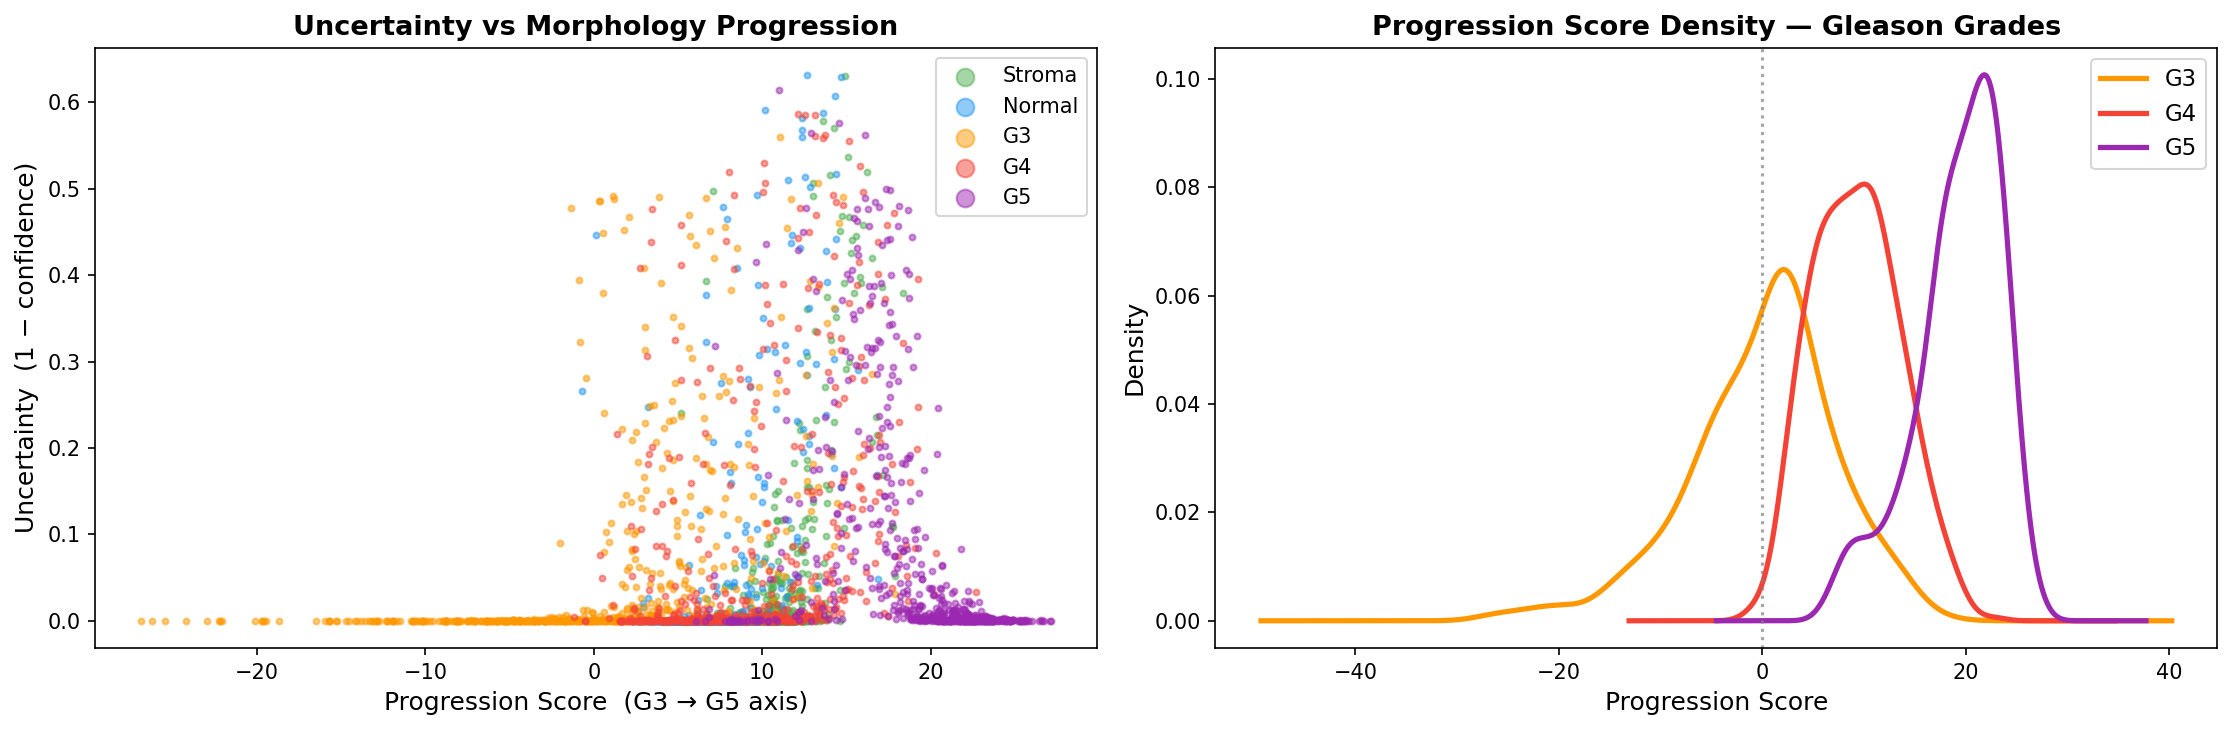
\includegraphics[width=0.80\textwidth]{figures/uncertainty_vs_progression.png}
\caption{Model prediction uncertainty plotted against progression score for all
patches. Uncertainty is measured as Shannon entropy over the five class
probabilities. Patches near the middle of the progression axis, corresponding
to grade 4, have the highest uncertainty.}
\label{fig:uncertainty}
\end{figure}

% ─────────────────────────────────────────────────────────────────────────────
\section{Generalisability and Robustness Across Imaging Domains}
% ─────────────────────────────────────────────────────────────────────────────

\subsection{Joint Visualisation of All Cohorts}

We fitted a single UMAP projection to all 3000 patches from all three cohorts
together. The result is shown in Figure~\ref{fig:joint_umap}. Looking at the
map coloured by tissue class, the grade ordering is still visible. However,
when the same map is coloured by cohort, a degree of cohort-level separation is
apparent, particularly for some tissue classes. The class silhouette score (0.163)
is larger than the domain silhouette score (0.004), indicating that class
structure is stronger than cohort structure overall.

This result should not be over-interpreted. A silhouette score of 0.163 is moderate,
not strong. It indicates partial rather than well-defined separation, meaning a
meaningful portion of patches from different classes overlap in the feature space.
The fact that class structure dominates over domain structure is a positive signal,
but the cross-domain classification results below demonstrate that the cohort
influence is still large enough to cause severe degradation in practice.

\begin{figure}[H]
\centering
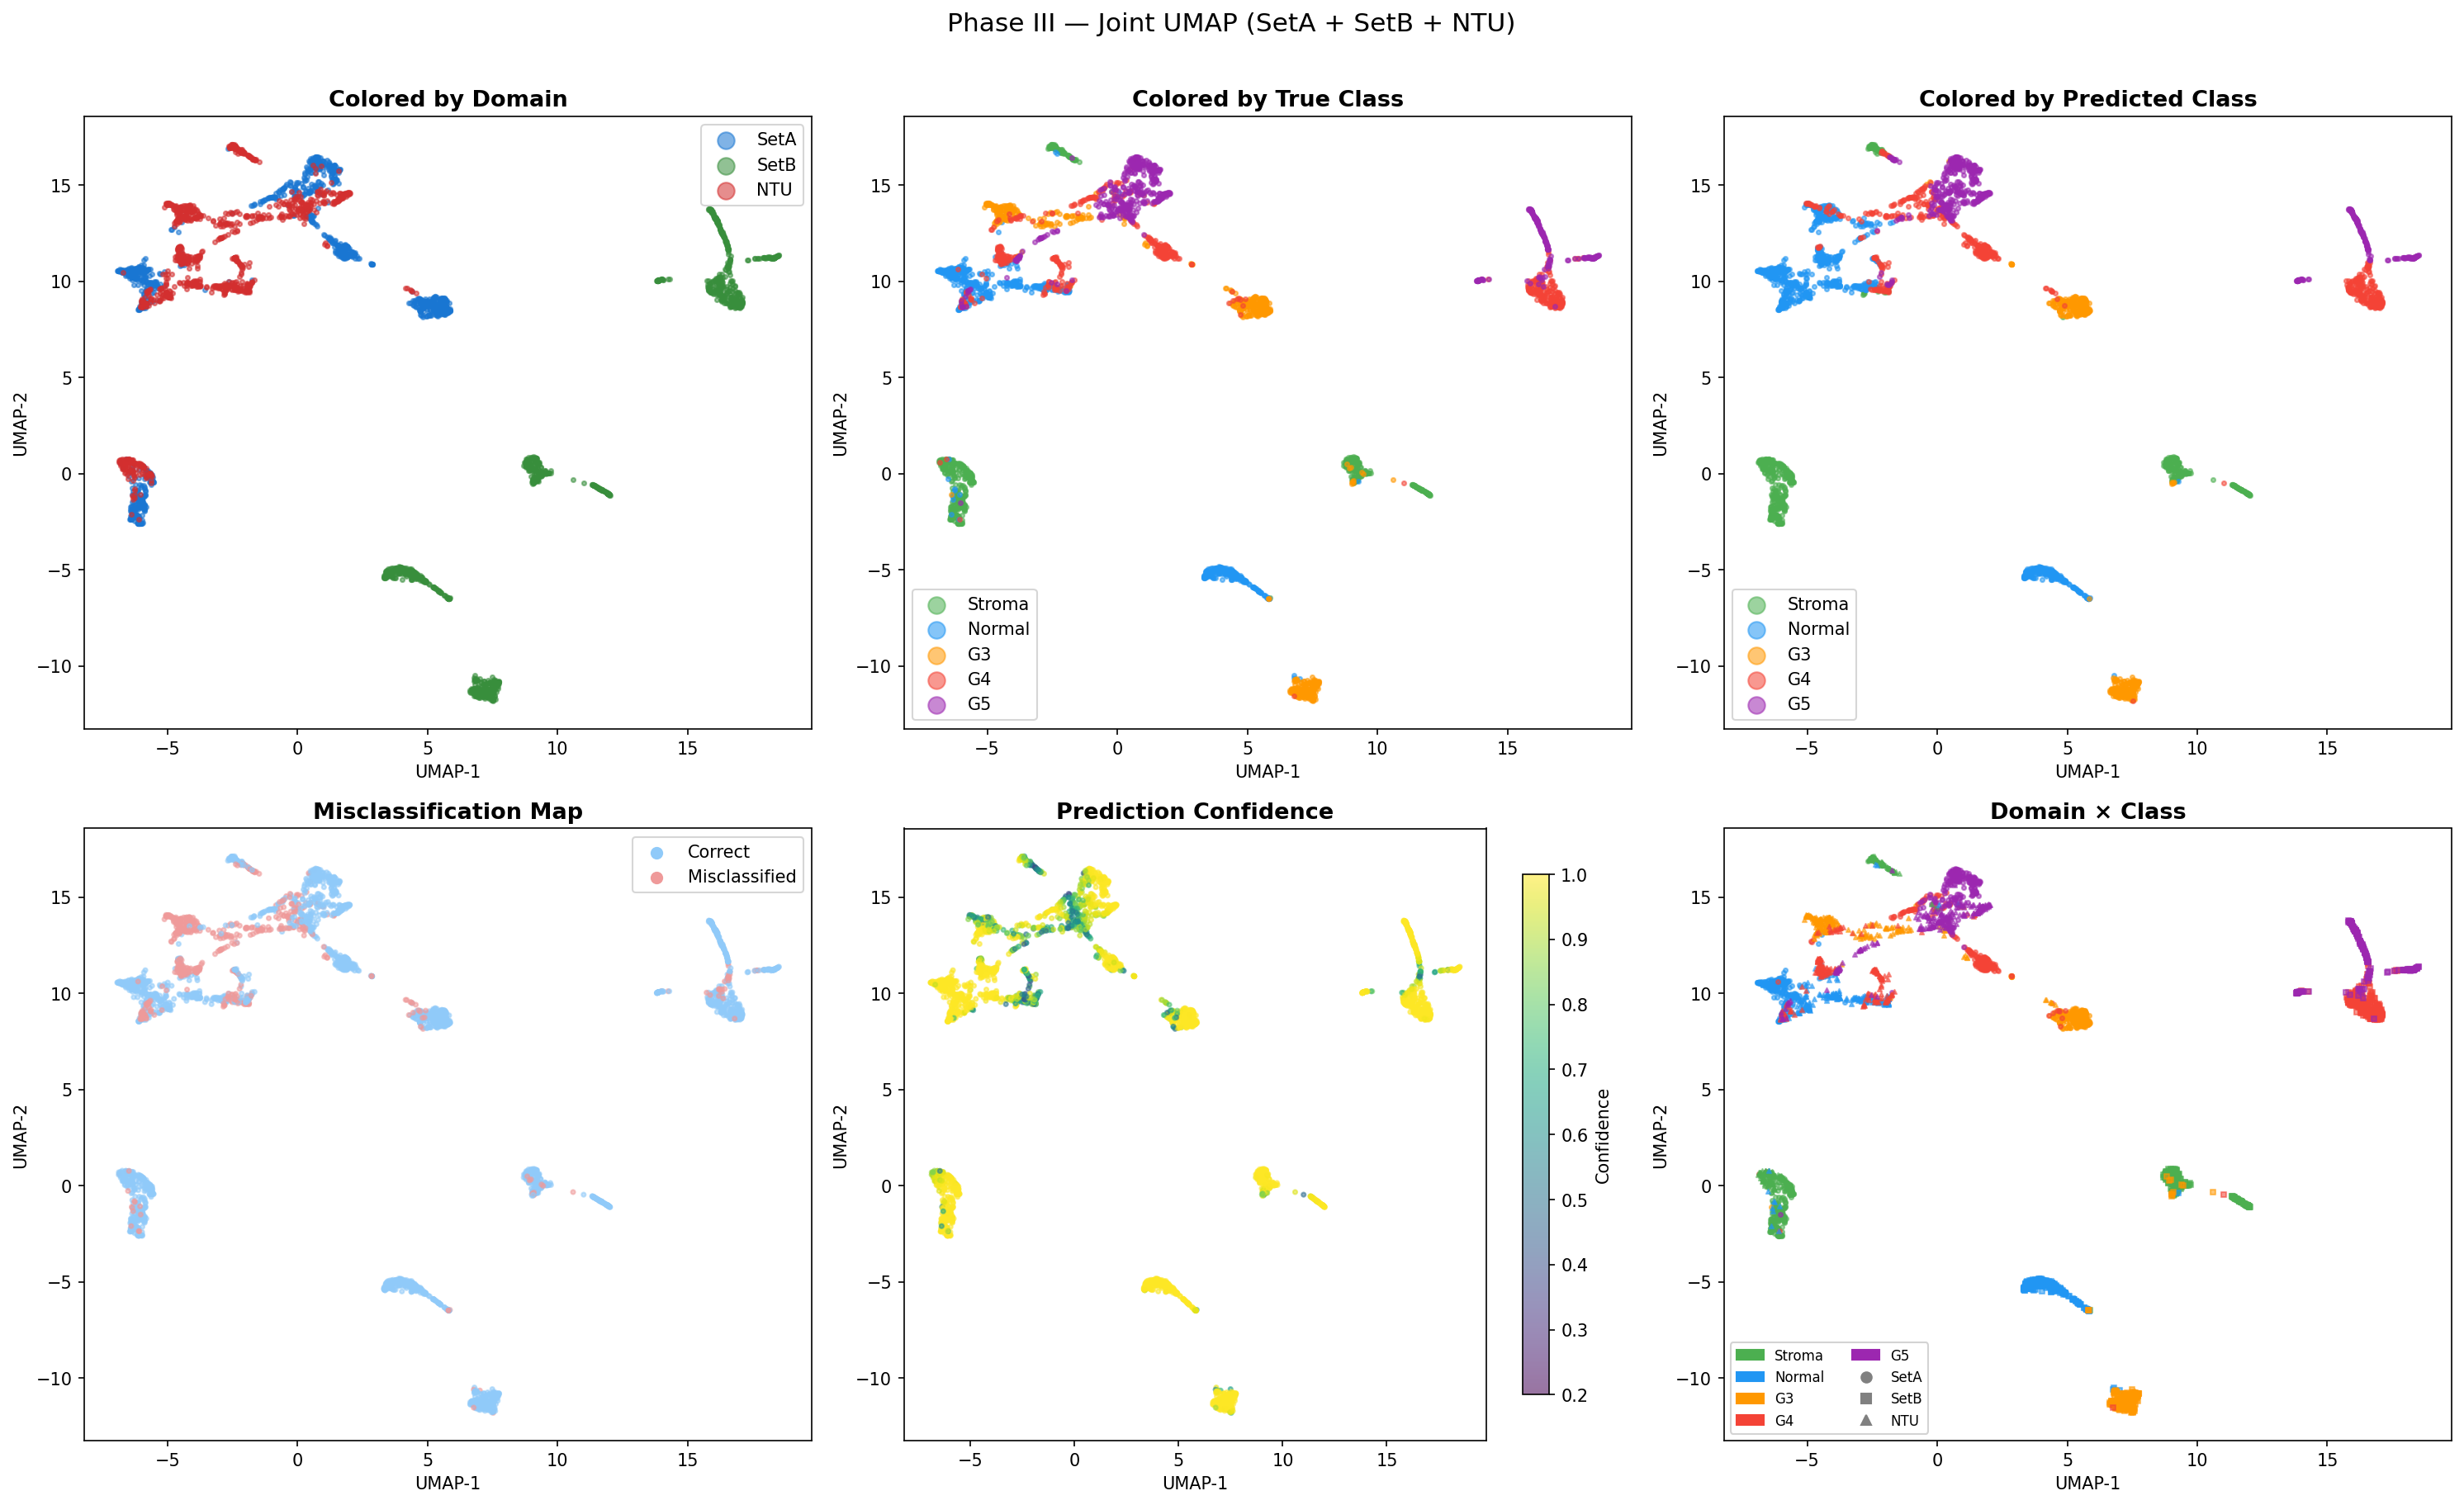
\includegraphics[width=0.92\textwidth]{figures/joint_umap_6panel.png}
\caption{Joint UMAP projection of all 3000 patches coloured in six different
ways. The class silhouette score (0.163) exceeds the domain silhouette score
(0.004), indicating that the learned representations cluster primarily by tissue
biology rather than by imaging cohort. However, a silhouette of 0.163 reflects
moderate rather than clean separation. Panels show colouring by class, cohort,
grade, confidence, progression score, and transition status.}
\label{fig:joint_umap}
\end{figure}

\subsection{Symmetric Cross-Domain Evaluation}

A critical test of generalisation is to apply a model trained on one cohort to
patches from a different cohort. Table~\ref{tab:crossdomain} shows the results
of all four within- and cross-cohort evaluations, along with performance on the
NTU external cohort.

\begin{table}[H]
\centering
\caption{Summary of classification performance under all evaluation conditions.
In-domain rows use the same cohort for training and testing. Cross-cohort rows
apply a model trained on one cohort to the test set of the other. The last row
shows performance on the NTU external cohort using the Cohort A model.}
\label{tab:crossdomain}
\begin{tabular}{llcc}
\toprule
\textbf{Model trained on} & \textbf{Tested on} & \textbf{Accuracy} & \textbf{Macro F1} \\
\midrule
Cohort A & Cohort A & 94.5\% & 94.4\% \\
Cohort B & Cohort B & 95.4\% & 95.4\% \\
Cohort A & Cohort B & 50.5\% & 39.6\% \\
Cohort B & Cohort A & 57.1\% & 55.8\% \\
Cohort A & NTU      & 50.2\% & 45.7\% \\
\bottomrule
\end{tabular}
\end{table}

The performance drop when crossing cohorts is large. Applying the Cohort A model
to Cohort B reduces macro F1 from 94.4 to 39.6 percent, a drop of 54.8 percentage
points. Applying the Cohort B model to Cohort A reduces macro F1 from 95.4 to
55.8 percent, a drop of 39.5 percentage points. The cross-cohort performance is
comparable to or worse than the performance on the NTU external cohort, even
though Cohort A and Cohort B nominally come from the same broader study.

The confusion matrices for all four evaluations are shown in Figure~\ref{fig:crossdomain}.
The in-domain panels show the expected strong diagonal. The cross-domain panels
show that the models concentrate most predictions in a small number of classes
rather than distributing them correctly across all five.

\begin{figure}[H]
\centering
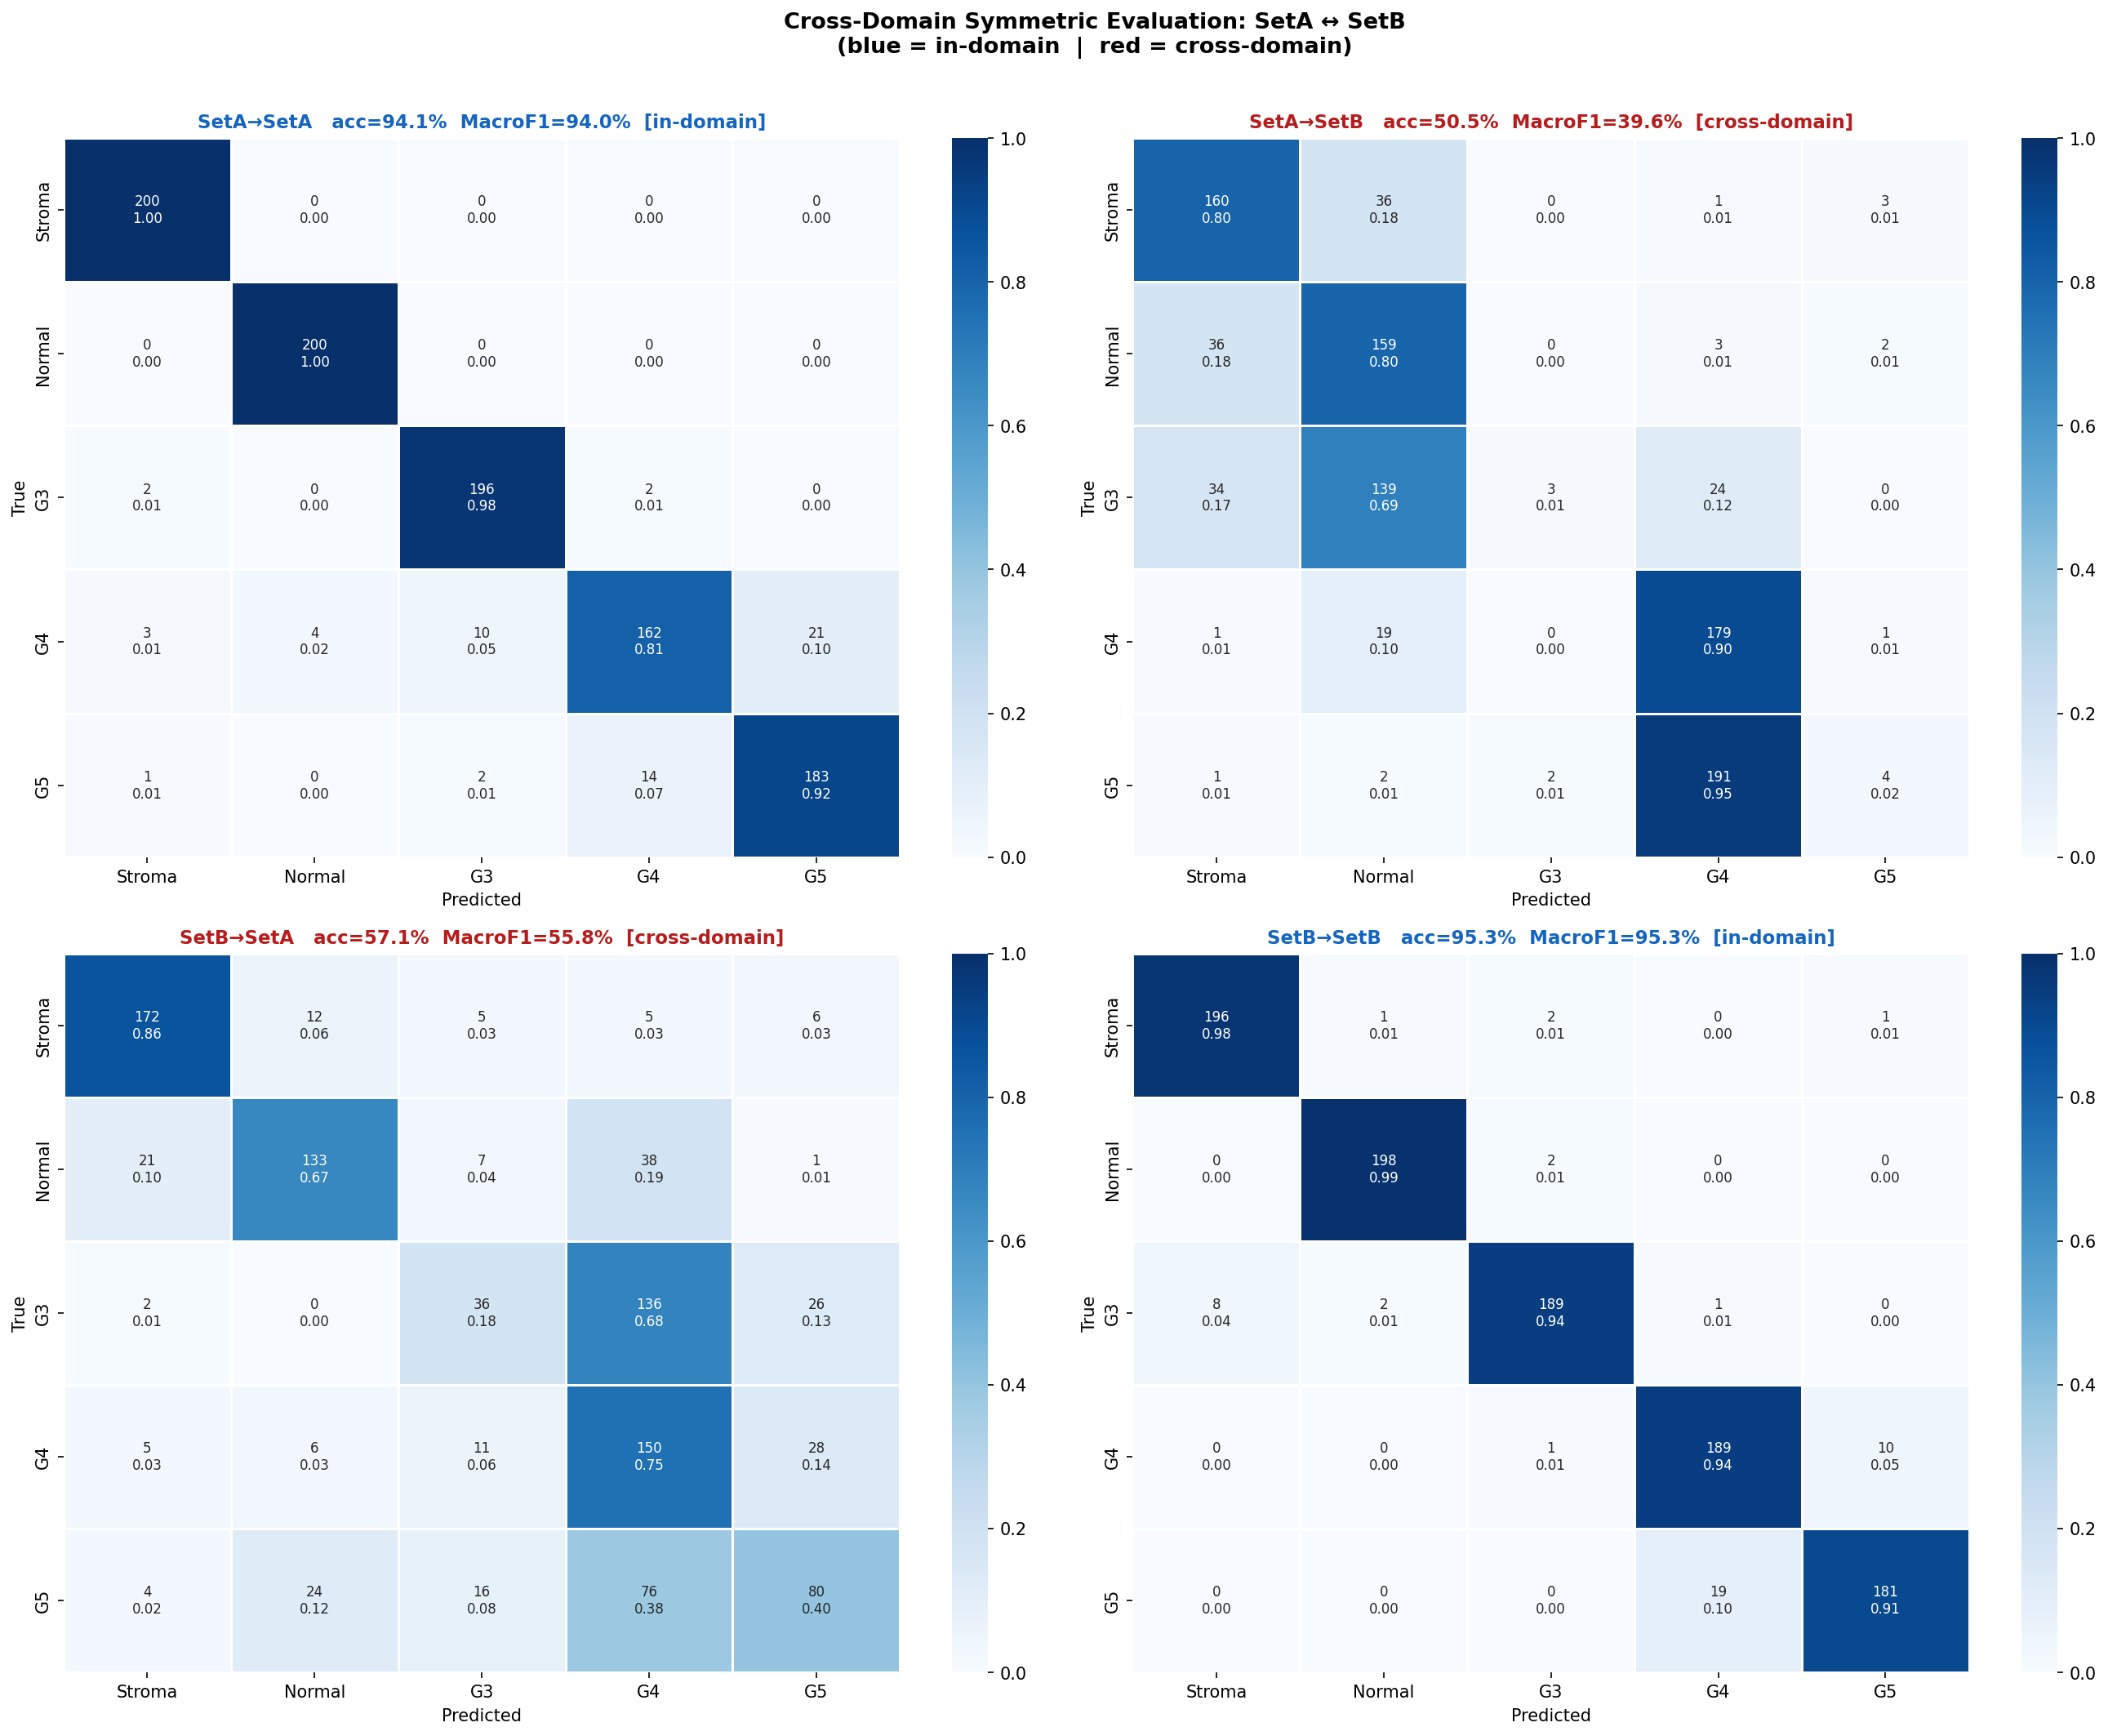
\includegraphics[width=\textwidth]{figures/cross_domain.png}
\caption{Confusion matrices for all four cross-cohort evaluations. In-domain
evaluations are shown in blue. Cross-cohort evaluations are shown in red. Each
cell shows the raw count and the row-normalised fraction. The cross-cohort
matrices show collapsed predictions concentrated in a few classes rather than
the correct grade distribution.}
\label{fig:crossdomain}
\end{figure}

\subsection{Per-Class Recall Breakdown}

Figure~\ref{fig:recall} shows per-class recall for all three evaluation domains
using the Cohort A model. Stroma and Normal are recalled at around 86 and 76
percent respectively on NTU. Grade 3, however, is recalled at 0 percent on NTU.
All 200 grade 3 NTU patches were misclassified, with 62.5 percent predicted as
Normal and 33.5 percent as grade 4.

This complete failure on NTU grade 3 is particularly striking. One hypothesis
worth investigating is a label-encoding mismatch between cohorts. If the NTU
dataset used a different label indexing convention during preparation (for instance,
a zero-indexed scheme mapping grade 3 to label 0, versus a one-indexed scheme
mapping grade 3 to label 1), then what appears visually as grade 3 tissue in NTU
may have been assigned a different numerical target than the model expects. A
nearest-neighbour inspection of the misclassified NTU grade 3 patches in feature
space confirms that their closest neighbours from training data are largely Normal
and grade 4 patches, consistent with both a genuine visual difference and a
possible label shift. This should be investigated before drawing conclusions about
the biological cause of the failure.

\begin{figure}[H]
\centering
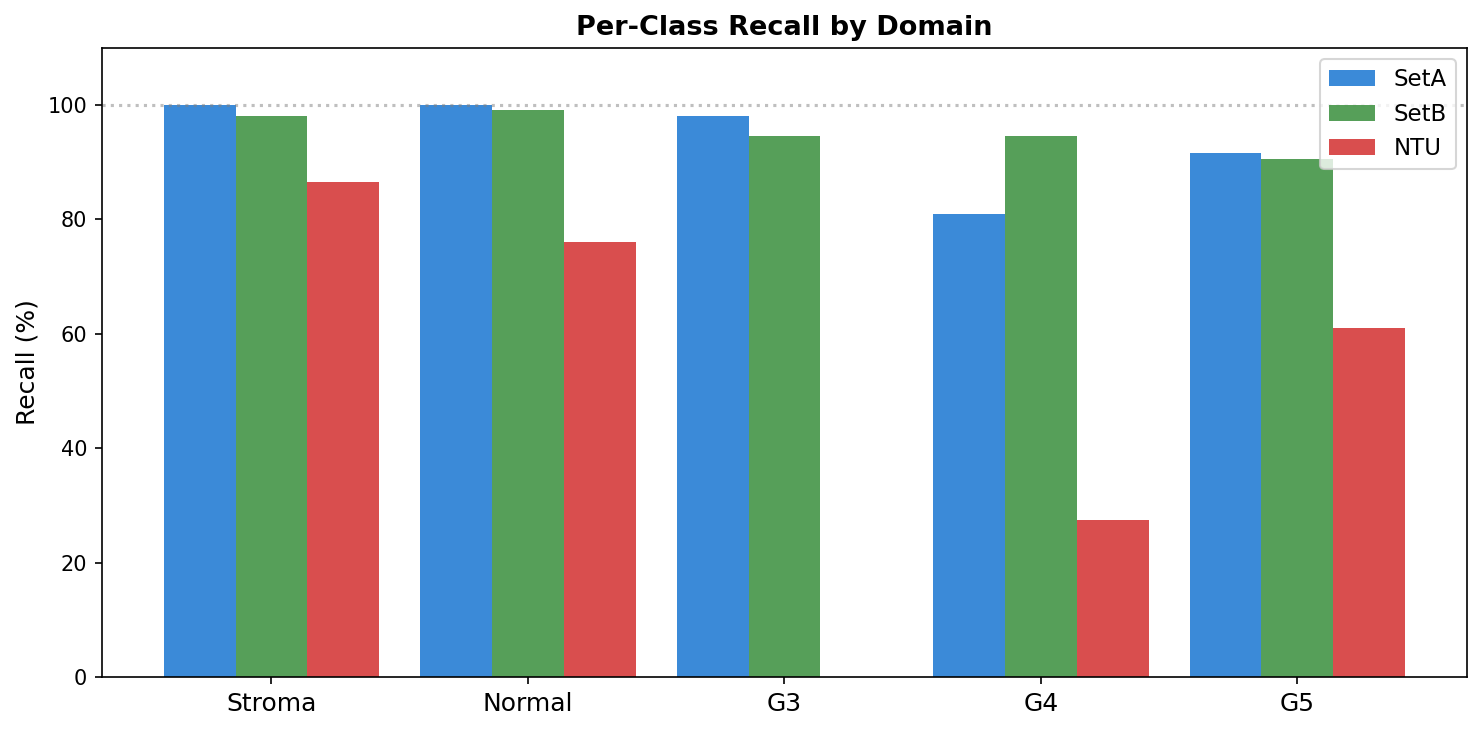
\includegraphics[width=0.85\textwidth]{figures/recall_by_domain.png}
\caption{Per-class recall for all three evaluation cohorts using the Cohort A
model. Stroma and Normal retain reasonable recall on NTU, but grade 3 recall
drops to zero. The grade 4 recall also degrades substantially on the NTU cohort.}
\label{fig:recall}
\end{figure}

\subsection{Stain Normalisation}

To investigate whether colour differences between cohorts drive the performance gap,
we applied Reinhard stain normalisation \citep{reinhard2001} to all NTU patches.
This method transfers the mean and standard deviation of the LAB colour channels
from a reference set of Cohort A patches to each NTU patch before inference.

The normalisation produced negligible improvement. Macro F1 increased by 0.27
percentage points (from 45.73 to 46.00 percent) and overall accuracy increased
by 0.20 percentage points. This result indicates that the performance gap is not
primarily driven by first-order colour statistics. However, non-recovery from
Reinhard normalisation does not rule out colour as a contributing factor entirely.
It only means that matching global LAB channel means and standard deviations is
insufficient. Local staining variation, texture-level colour patterns, and
differences in tissue processing would not be corrected by this operation.

\subsection{Calibration Under Domain Shift}

Table~\ref{tab:calibration} shows the calibration statistics for each evaluation
cohort. The Expected Calibration Error (ECE) measures how well the model's
confidence aligns with its actual accuracy. A well-calibrated model that says it
is 90 percent confident should be correct around 90 percent of the time. These
ECE comparisons are descriptive; no bootstrap confidence intervals were computed,
so small differences between cohorts should not be over-interpreted.

\begin{table}[H]
\centering
\caption{Calibration summary for each evaluation cohort. Expected Calibration
Error is computed using 15 equal-width confidence bins. Lower ECE indicates
better calibration. The last two columns show mean confidence on correct and
incorrect predictions respectively.}
\label{tab:calibration}
\begin{tabular}{lccc}
\toprule
\textbf{Cohort} & \textbf{ECE} & \textbf{Mean conf.\ when correct} & \textbf{Mean conf.\ when wrong} \\
\midrule
Cohort A & 0.030 & 0.977 & 0.789 \\
Cohort B & 0.032 & 0.992 & 0.839 \\
NTU      & 0.370 & 0.907 & 0.845 \\
\bottomrule
\end{tabular}
\end{table}

On the training cohorts, the model is well-calibrated with ECE values below 0.033.
On NTU, the ECE jumps to 0.370. What makes this particularly concerning is that
the mean confidence when the model is wrong on NTU is 0.845. The model makes
confident incorrect predictions at nearly the same confidence level as correct
ones. In a clinical setting, this would mean that a clinician relying on the
model's confidence score could not detect when the model was about to make a
dangerous grading error.

% ─────────────────────────────────────────────────────────────────────────────
\section{Structural Interpretation of Tissue Architecture}
% ─────────────────────────────────────────────────────────────────────────────

\subsection{Motivation}

While the learned feature space shows that the network builds a meaningful
representation of Gleason grades, it does not explain what physical aspects of
tissue structure it has learned to use. To address this, we extracted twelve
hand-crafted structural features from the raw images and examined whether they
align with the grade ordering found in the neural network feature space.

This analysis serves two purposes. First, it provides a biologically interpretable
explanation for the progression axis found in the feature space. Second, the
Structural Accessibility Index introduced below has potential relevance to drug
delivery, since poorly differentiated high-grade tumours are known to present
physical barriers to drug penetration \citep{minchinton2006}.

\subsection{Feature Extraction}

Haematoxylin and eosin staining separates two main tissue components. Haematoxylin
stains cell nuclei blue-purple and eosin stains the surrounding tissue pink. We
used colour deconvolution following the method of \citet{ruifrok2001} to separate
these two channels. This gives an estimate of how much haematoxylin and eosin are
present at each pixel.

From these separated channels we derived twelve features. Lumen fraction is the
proportion of pixels that are pale enough to represent open glandular space.
Nuclei area fraction is the proportion of pixels with strong haematoxylin signal.
Epithelial fraction and stroma fraction are computed from which stain dominates
at each pixel. The epithelial-to-stroma ratio divides these two quantities.
Cellular crowding index divides nuclei fraction by the available non-lumen tissue
area. Texture entropy is computed from the grey-level histogram. The remaining
four features are Haralick texture statistics derived from a Grey-Level
Co-occurrence Matrix \citep{haralick1973}, capturing energy, contrast, homogeneity,
and correlation in the spatial arrangement of grey levels.

\subsection{Correlation with Grade Progression}

Figure~\ref{fig:spearman} shows the Spearman rank correlation between each feature
and the progression score for grade 3, 4, and 5 patches. Nine of twelve features
have statistically significant correlations after Bonferroni correction
($\alpha / 12 = 0.00417$). Table~\ref{tab:spearman} lists all twelve features with
their correlation coefficients and significance status.

\begin{figure}[H]
\centering

\includegraphics[width=0.80\textwidth]{figures/spearman_bar.png}
\caption{Spearman rank correlation between each structural feature and the grade
progression score, computed on grade 3, 4, and 5 patches. Negative values indicate
the feature decreases as grade increases. Bars are coloured by significance after
Bonferroni correction at the $\alpha/12 = 0.00417$ threshold. GLCM correlation
and lumen fraction are the strongest individual predictors.}
\label{fig:spearman}
\end{figure}

\begin{table}[H]
\centering
\caption{Spearman rank correlations between structural features and the progression
score for grades 3 to 5. Features marked with an asterisk are significant at the
Bonferroni-corrected threshold ($\alpha/12 = 0.00417$). Positive values indicate
the feature increases from grade 3 to grade 5.}
\label{tab:spearman}
\begin{tabular}{lcc}
\toprule
\textbf{Feature} & \textbf{Spearman $\rho$} & \textbf{Significant} \\
\midrule
GLCM Correlation    & $-$0.477 & Yes* \\
Lumen Fraction      & $-$0.434 & Yes* \\
SAI                 & $-$0.408 & Yes* \\
GLCM Homogeneity    & $-$0.373 & Yes* \\
GLCM Contrast       & $+$0.348 & Yes* \\
Nuclei Fraction     & $+$0.289 & Yes* \\
Epithelial Fraction & $+$0.286 & Yes* \\
Epi-Stroma Ratio    & $+$0.206 & Yes* \\
Crowding Index      & $+$0.202 & Yes* \\
Texture Entropy     & $+$0.054 & No  \\
GLCM Energy         & $-$0.033 & No  \\
Stroma Fraction     & $+$0.004 & No  \\
\bottomrule
\end{tabular}
\end{table}

Texture entropy has a raw $p$-value of 0.021, which would appear significant at
the uncorrected $\alpha = 0.05$ level. After Bonferroni correction the adjusted
$p$-value is 0.251, which is well above the threshold. Reporting this feature as
significant without correction would be misleading given the twelve features tested
simultaneously. Stroma fraction and GLCM energy show negligible correlations and
are not significant at any reasonable threshold.

The direction of the significant correlations makes biological sense. Lumen fraction
decreases as grade increases because well-formed open glands (grade 3) are replaced
by fused or absent glands (grade 4 and 5). Nuclei fraction increases because
higher-grade tumours have more densely packed cells. GLCM homogeneity decreases
and contrast increases because higher-grade tissue has more irregular spatial
texture. Figure~\ref{fig:violin} shows the distribution of each feature across all
five tissue classes, confirming that the trends are consistent.

\begin{figure}[H]
\centering
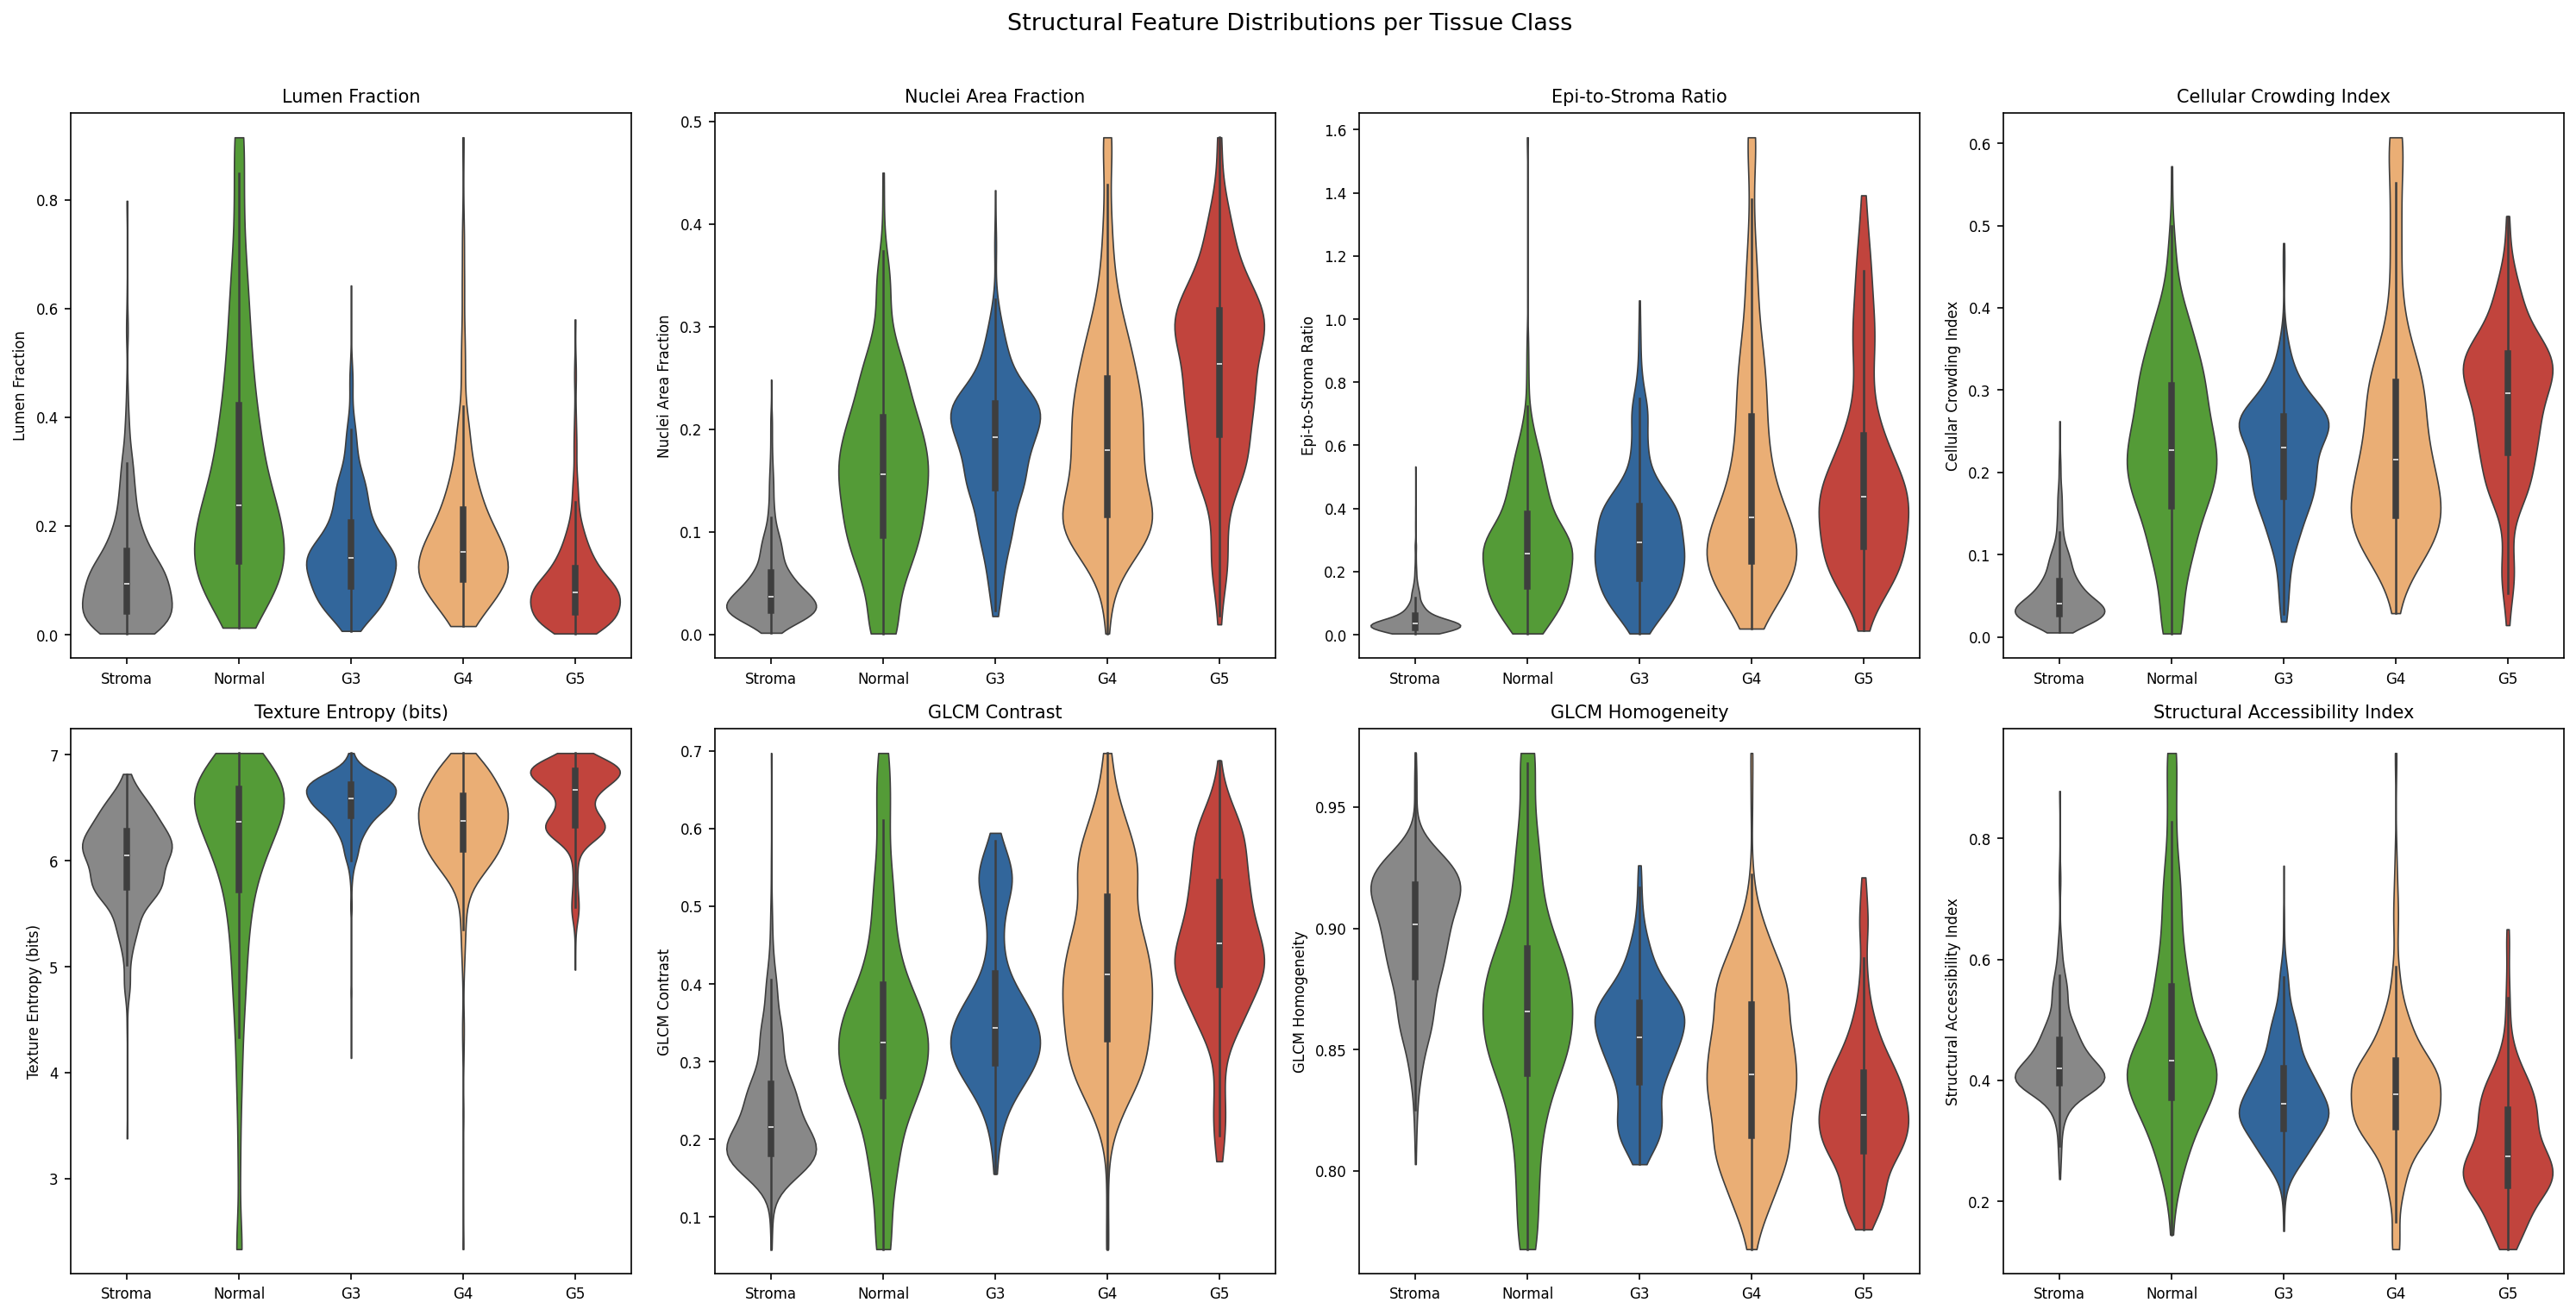
\includegraphics[width=\textwidth]{figures/violin.png}
\caption{Distribution of eight structural features across all five tissue classes.
Each violin shows the full distribution and an inner box-and-whisker plot. The
ordering from grade 3 to grade 5 is visible for lumen fraction, nuclei fraction,
cellular crowding index, and GLCM contrast.}
\label{fig:violin}
\end{figure}

\subsection{Kruskal-Wallis Tests Across All Five Classes}

To assess whether each feature discriminates among all five tissue classes, not
only the cancer grades, we applied Kruskal-Wallis tests across the full set of
3000 patches. All twelve features are significant at $p < 10^{-100}$, with
epithelial fraction achieving the largest test statistic ($H = 1490$) followed
by epithelial-to-stroma ratio ($H = 1403$) and nuclei fraction ($H = 1378$).
This confirms that every feature, including the three that are not significantly
correlated with the cancer-grade progression score, still captures meaningful
variation when benign tissue classes are included.

\subsection{Structural Accessibility Index}

We defined a Structural Accessibility Index (SAI) to quantify how physically
accessible a tissue patch is to a drug delivered through the bloodstream. The
index is a weighted combination of a normalised lumen fraction and the inverse
of a normalised nuclei fraction,

\begin{equation}
\text{SAI} = 0.6 \cdot \hat{L} + 0.4 \cdot (1 - \hat{N})
\end{equation}

where $\hat{L}$ is the lumen fraction and $\hat{N}$ is the nuclei area fraction,
both normalised to the range 0 to 1 across the full dataset. Lumen fraction
receives the larger weight because open glandular space represents the most direct
route for drug transport. Nuclei fraction receives the smaller weight because
dense nuclear packing indicates compact tissue that impedes diffusion. Higher SAI
means more open, accessible tissue.

Figure~\ref{fig:sai} shows the SAI distribution. The median SAI decreases from
grade 3 (0.374) to grade 5 (0.289), confirming that higher-grade tumours are
structurally less accessible. The Spearman correlation between SAI and progression
score is $-0.408$ (p $< 10^{-72}$).

\begin{figure}[H]
\centering

\includegraphics[width=0.90\textwidth]{figures/sai_deepdive.png}
\caption{Left panel shows SAI plotted against the progression score for grade 3,
4, and 5 patches. The downward trend confirms that higher-grade tissue is
structurally less accessible. Right panel shows SAI distributions as box plots
for all five tissue classes.}
\label{fig:sai}
\end{figure}

\subsection{SAI Weight Sensitivity}

The 0.6 / 0.4 weighting between lumen fraction and the inverse nuclei fraction is
a design choice. To confirm that the results are not sensitive to this choice,
we evaluated four weight combinations spanning from equal weighting (0.5 / 0.5)
to strongly lumen-dominated (0.8 / 0.2). The results are shown in
Table~\ref{tab:sai_sensitivity}.

\begin{table}[H]
\centering
\caption{SAI weight sensitivity analysis. Spearman $\rho$ between SAI and the
progression score, and mean SAI per cancer grade, for four weight combinations.
The Spearman correlation varies by less than 0.06 across all combinations and
the direction remains consistently negative.}
\label{tab:sai_sensitivity}
\begin{tabular}{cccccc}
\toprule
$w_L$ & $w_N$ & \textbf{Spearman $\rho$} & \textbf{G3 mean} & \textbf{G4 mean} & \textbf{G5 mean} \\
\midrule
0.5 & 0.5 & $-$0.387 & 0.428 & 0.433 & 0.337 \\
0.6 & 0.4 & $-$0.408 & 0.374 & 0.384 & 0.289 \\
0.7 & 0.3 & $-$0.427 & 0.321 & 0.335 & 0.241 \\
0.8 & 0.2 & $-$0.441 & 0.267 & 0.286 & 0.193 \\
\bottomrule
\end{tabular}
\end{table}

The Spearman correlation ranges from $-0.387$ to $-0.441$ across all four
combinations. The direction is consistently negative and the grade ordering
G3 $>$ G4 $>$ G5 is preserved in every case. The selected weights
($w_L = 0.6$, $w_N = 0.4$) are not a special case; any reasonable lumen-dominant
weighting yields the same qualitative conclusion.

\subsection{Grade 4 as a Heterogeneous Transition Region}

A Levene variance test confirmed that the SAI variance for grade 4 is
significantly different from grade 3 and grade 5 (F $= 10.74$, p $< 0.001$).
Grade 4 has a standard deviation of 0.115, compared to 0.081 for grade 3 and
0.095 for grade 5. This means that grade 4 patches span both the low-SAI
(compact, high-grade-like) and high-SAI (open, low-grade-like) ends of the
accessibility range. This is consistent with the known biology of Gleason grade 4,
which includes multiple architectural subtypes such as cribriform glands, fused
glands, and poorly formed glands that are structurally very different from each
other.

\subsection{Domain Robustness of Structural Features}

To test whether the structural features are stable across imaging cohorts, we
applied a Kruskal-Wallis test within each grade, comparing feature distributions
across all three cohorts. If a feature shows no significant difference between
cohorts within the same grade, it is domain-robust in that grade.

Of the twelve features tested, only one was domain-robust at grade 4, which is
SAI (p $= 0.29$). All eleven other features showed significant differences across
cohorts at both grade 3 and grade 5. Figure~\ref{fig:sai_robust} illustrates
the SAI distribution across cohorts for each grade. The grade 4 SAI distributions
from all three cohorts overlap substantially, while the grade 3 and grade 5 SAI
distributions show cohort-level shifts.

\begin{figure}[H]
\centering
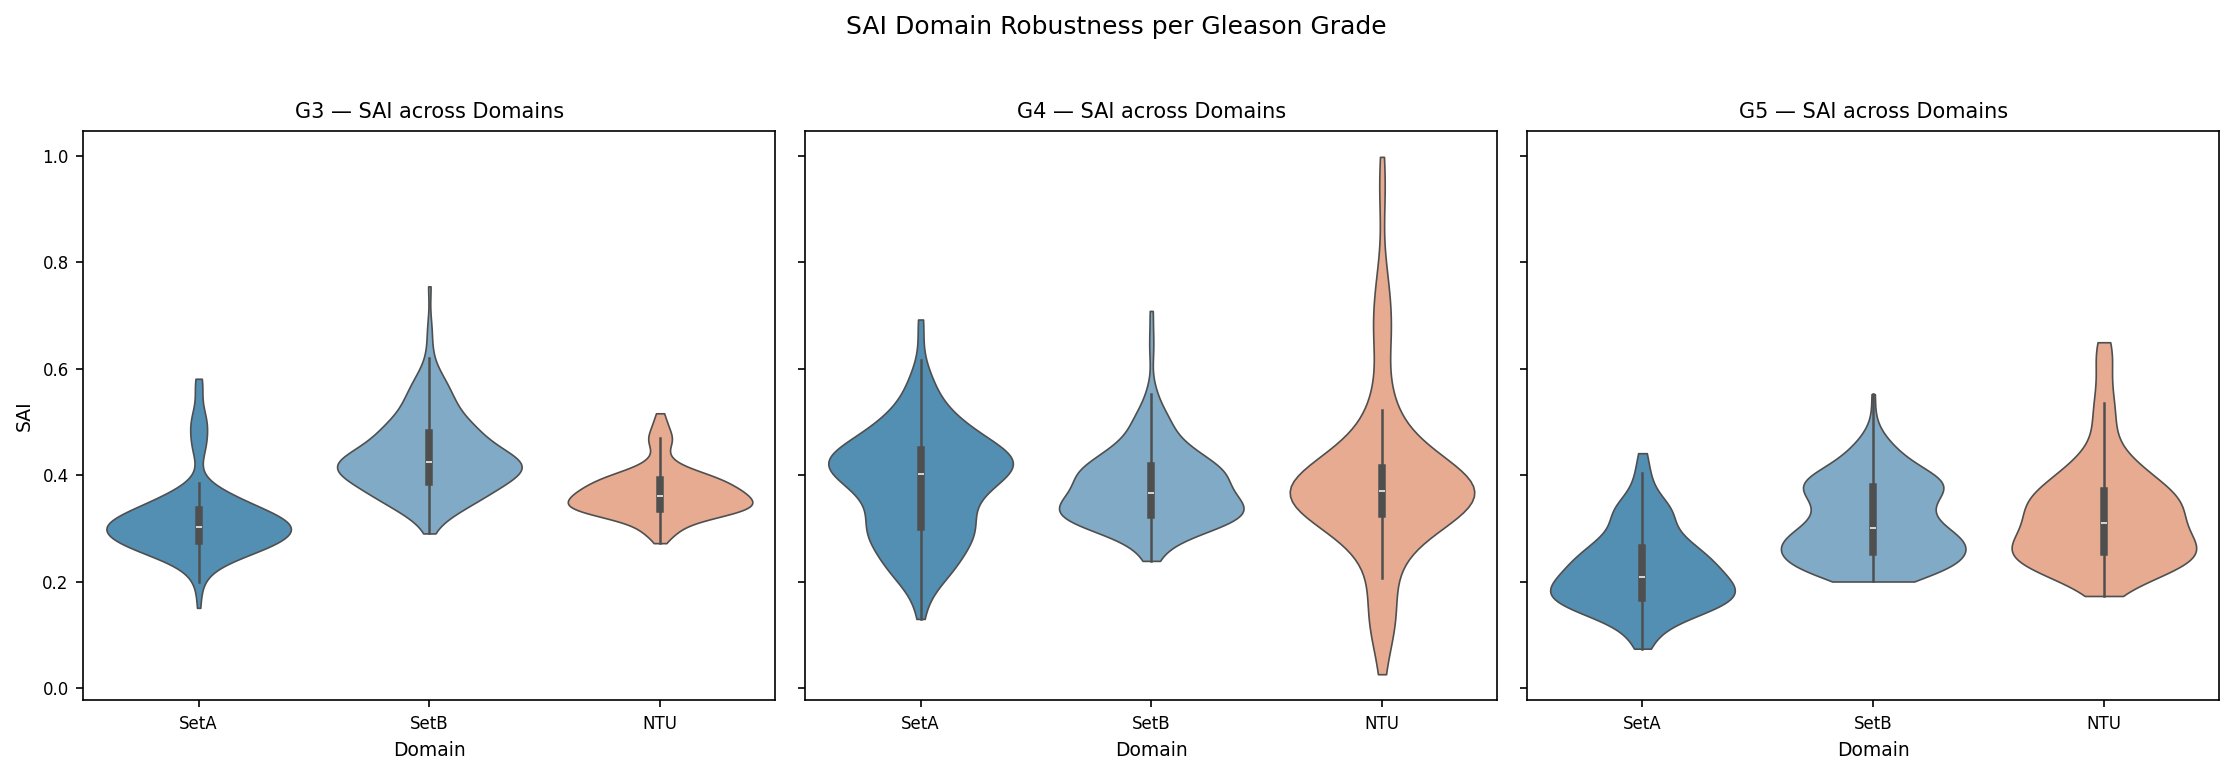
\includegraphics[width=0.90\textwidth]{figures/sai_robustness.png}
\caption{SAI distributions for grades 3, 4, and 5 across all three imaging cohorts.
Grade 4 SAI is the only configuration that is not significantly different across
cohorts (Kruskal-Wallis p $= 0.29$). Grade 3 and grade 5 SAI distributions show
cohort-level shifts, indicating that scanner and staining differences affect
absolute feature values.}
\label{fig:sai_robust}
\end{figure}

\subsection{Ablation Study}

To assess how much predictive power each feature has individually, we fitted a
linear regression model using each feature alone as a predictor of the progression
score and evaluated performance using five-fold cross-validation. All six evaluated
features produced negative cross-validated $R^2$ values. Results are shown in
Table~\ref{tab:ablation}.

\begin{table}[H]
\centering
\caption{Five-fold cross-validated $R^2$ for individual feature linear regression
on the grade progression score. All values are negative, indicating that no single
feature is sufficient for linear prediction.}
\label{tab:ablation}
\begin{tabular}{lc}
\toprule
\textbf{Feature} & \textbf{CV $R^2$} \\
\midrule
GLCM Homogeneity  & $-$0.150 \\
GLCM Contrast     & $-$0.190 \\
GLCM Correlation  & $-$0.202 \\
SAI               & $-$0.325 \\
Epithelial Frac.  & $-$0.340 \\
Nuclei Fraction   & $-$0.368 \\
\bottomrule
\end{tabular}
\end{table}

Negative cross-validated $R^2$ means the model predicts the progression score
worse than simply guessing the training-set mean. This does not contradict the
Spearman correlations, which measure monotonic rank agreement and do not require
a linear relationship. The progression score is constructed from 1408 neural
network dimensions. Individual hand-crafted features capture only a narrow slice
of the information encoded in that space. The Spearman correlations demonstrate
that the features are biologically aligned with grade ordering. The ablation results
demonstrate that this alignment is insufficient for linear prediction of a complex
multi-dimensional latent score.

% ─────────────────────────────────────────────────────────────────────────────
\section{Discussion}
% ─────────────────────────────────────────────────────────────────────────────

\subsection{What the Results Show}

This study demonstrates that a standard convolutional neural network can classify
prostate tissue patches at a high level of accuracy when training and test data
come from the same imaging cohort. The model learns representations that reflect
the biological ordering of Gleason grades, with a continuous progression from
grade 3 to grade 5 visible in the feature space without any explicit supervision
of that ordering. The grade 4 cluster is broader and more dispersed than the
other cancer grades, which is consistent with the known architectural heterogeneity
of this intermediate grade.

The structural feature analysis confirms that the grade ordering captured by the
network corresponds to real measurable changes in tissue architecture. Lumen
fraction decreases and nuclear crowding increases monotonically from grade 3 to
grade 5, exactly as expected from the definitions of the Gleason grades. Nine of
twelve structural features show statistically significant Spearman correlations with
the progression score after Bonferroni correction, and the Kruskal-Wallis tests
confirm that all features discriminate among all five tissue classes. The SAI
provides a single composite summary of structural accessibility that could
potentially be used to estimate drug penetration capacity from a routine biopsy
image.

\subsection{The Domain Generalisation Problem}

The central finding of concern is the magnitude of performance loss when models
are applied across imaging sites. A drop of 54.8 percentage points in macro F1
when applying the Cohort A model to Cohort B is not a small calibration shift.
It represents a near-complete failure of the classifier. The model appears to
have learned a mixture of biological signal and cohort-specific imaging
characteristics that are inseparable from each other when trained on a single cohort.

The fact that Cohort A performs better on the NTU external cohort (45.7 percent)
than on Cohort B (39.6 percent) is counterintuitive given that NTU is a genuinely
external dataset. This suggests that the imaging characteristics of Cohort B are
more different from Cohort A than the imaging characteristics of NTU. It also
means that using two nominally paired cohorts does not guarantee that a model will
generalise between them.

The complete failure on NTU grade 3 patches, where every single grade 3 patch was
misclassified, is the most clinically alarming finding. As noted in Section 6.3,
a label-encoding mismatch between cohorts is one possible contributing factor and
should be investigated before attributing the failure entirely to visual domain
shift. Regardless of the cause, if this model were deployed at the NTU site, grade
3 tumours would be systematically misclassified as either Normal tissue or grade 4.
Combined with the finding that the model remains confident even when wrong (mean
confidence of 0.845 on incorrect NTU predictions), a clinician would receive
high-confidence wrong grades with no warning signal.

\subsection{Limitations}

The models were trained with only two source cohorts. Exposure to a larger variety
of imaging protocols during training, either through multi-site datasets or through
aggressive stain augmentation, would likely improve domain robustness. The Reinhard
colour transfer used here operates on global image statistics and cannot account for
local staining variability or differences in tissue processing.

The progression axis is defined by the grade 3 and grade 5 centroids, which means
the ordering of these two grades is guaranteed rather than discovered. External
validation on held-out data would be needed to confirm that the axis captures a
genuine biological latent variable rather than an artefact of the training cohort
geometry.

The structural features were computed from individual patches without spatial context.
Features such as gland density and the arrangement of grade 4 and grade 5 regions
within a biopsy core would require whole-slide-level analysis.

% ─────────────────────────────────────────────────────────────────────────────
\section{Conclusion}
% ─────────────────────────────────────────────────────────────────────────────

We have shown that a convolutional neural network trained on prostate tissue
patches can achieve high classification accuracy within a single imaging cohort
and that the internal representations it learns reflect the biological ordering
of Gleason grades. Structural features extracted from the raw images confirm this
alignment at the level of measurable tissue architecture. Nine of twelve features
show statistically significant Spearman correlations with the grade progression
score after Bonferroni correction. The Structural Accessibility Index, combining
lumen openness and nuclear density, provides a biologically motivated summary of
tissue compactness that decreases monotonically from grade 3 to grade 5, and its
direction is robust to the choice of component weights.

However, the models fail to generalise reliably across imaging sites. Performance
drops of up to 54.8 percentage points, combined with high-confidence wrong
predictions on external data, indicate that the models have absorbed cohort-specific
imaging characteristics that are not portable to new sites. Grade 3 tissue from an
external cohort was misclassified at 100 percent, a finding that would be clinically
unacceptable regardless of whether its cause is visual domain shift, a label-encoding
discrepancy, or both.

Solving the domain shift problem is the most important next step. Approaches worth
exploring include training on a wider range of imaging cohorts, using domain
adversarial training to explicitly suppress cohort-specific features, applying
stronger stain augmentation, and using foundation models pretrained on large and
diverse pathology datasets. Until robust cross-domain performance is demonstrated,
these models should be used only as decision support tools in settings where their
training data closely matches the target imaging environment.

% ─────────────────────────────────────────────────────────────────────────────
\bibliographystyle{abbrvnat}
\bibliography{references}

\end{document}
